\documentclass[twoside]{book}

% Packages required by doxygen
\usepackage{fixltx2e}
\usepackage{calc}
\usepackage{doxygen}
\usepackage[export]{adjustbox} % also loads graphicx
\usepackage{graphicx}
\usepackage[utf8]{inputenc}
\usepackage{makeidx}
\usepackage{multicol}
\usepackage{multirow}
\PassOptionsToPackage{warn}{textcomp}
\usepackage{textcomp}
\usepackage[nointegrals]{wasysym}
\usepackage[table]{xcolor}

% Font selection
\usepackage[T1]{fontenc}
\usepackage[scaled=.90]{helvet}
\usepackage{courier}
\usepackage{amssymb}
\usepackage{sectsty}
\renewcommand{\familydefault}{\sfdefault}
\allsectionsfont{%
  \fontseries{bc}\selectfont%
  \color{darkgray}%
}
\renewcommand{\DoxyLabelFont}{%
  \fontseries{bc}\selectfont%
  \color{darkgray}%
}
\newcommand{\+}{\discretionary{\mbox{\scriptsize$\hookleftarrow$}}{}{}}

% Page & text layout
\usepackage{geometry}
\geometry{%
  a4paper,%
  top=2.5cm,%
  bottom=2.5cm,%
  left=2.5cm,%
  right=2.5cm%
}
\tolerance=750
\hfuzz=15pt
\hbadness=750
\setlength{\emergencystretch}{15pt}
\setlength{\parindent}{0cm}
\setlength{\parskip}{3ex plus 2ex minus 2ex}
\makeatletter
\renewcommand{\paragraph}{%
  \@startsection{paragraph}{4}{0ex}{-1.0ex}{1.0ex}{%
    \normalfont\normalsize\bfseries\SS@parafont%
  }%
}
\renewcommand{\subparagraph}{%
  \@startsection{subparagraph}{5}{0ex}{-1.0ex}{1.0ex}{%
    \normalfont\normalsize\bfseries\SS@subparafont%
  }%
}
\makeatother

% Headers & footers
\usepackage{fancyhdr}
\pagestyle{fancyplain}
\fancyhead[LE]{\fancyplain{}{\bfseries\thepage}}
\fancyhead[CE]{\fancyplain{}{}}
\fancyhead[RE]{\fancyplain{}{\bfseries\leftmark}}
\fancyhead[LO]{\fancyplain{}{\bfseries\rightmark}}
\fancyhead[CO]{\fancyplain{}{}}
\fancyhead[RO]{\fancyplain{}{\bfseries\thepage}}
\fancyfoot[LE]{\fancyplain{}{}}
\fancyfoot[CE]{\fancyplain{}{}}
\fancyfoot[RE]{\fancyplain{}{\bfseries\scriptsize Generated by Doxygen }}
\fancyfoot[LO]{\fancyplain{}{\bfseries\scriptsize Generated by Doxygen }}
\fancyfoot[CO]{\fancyplain{}{}}
\fancyfoot[RO]{\fancyplain{}{}}
\renewcommand{\footrulewidth}{0.4pt}
\renewcommand{\chaptermark}[1]{%
  \markboth{#1}{}%
}
\renewcommand{\sectionmark}[1]{%
  \markright{\thesection\ #1}%
}

% Indices & bibliography
\usepackage{natbib}
\usepackage[titles]{tocloft}
\setcounter{tocdepth}{3}
\setcounter{secnumdepth}{5}
\makeindex

% Hyperlinks (required, but should be loaded last)
\usepackage{ifpdf}
\ifpdf
  \usepackage[pdftex,pagebackref=true]{hyperref}
\else
  \usepackage[ps2pdf,pagebackref=true]{hyperref}
\fi
\hypersetup{%
  colorlinks=true,%
  linkcolor=blue,%
  citecolor=blue,%
  unicode%
}

% Custom commands
\newcommand{\clearemptydoublepage}{%
  \newpage{\pagestyle{empty}\cleardoublepage}%
}

\usepackage{caption}
\captionsetup{labelsep=space,justification=centering,font={bf},singlelinecheck=off,skip=4pt,position=top}

%===== C O N T E N T S =====

\begin{document}

% Titlepage & ToC
\hypersetup{pageanchor=false,
             bookmarksnumbered=true,
             pdfencoding=unicode
            }
\pagenumbering{alph}
\begin{titlepage}
\vspace*{7cm}
\begin{center}%
{\Large Neo \\[1ex]\large 1.\+0 }\\
\vspace*{1cm}
{\large Generated by Doxygen 1.8.14}\\
\end{center}
\end{titlepage}
\clearemptydoublepage
\pagenumbering{roman}
\tableofcontents
\clearemptydoublepage
\pagenumbering{arabic}
\hypersetup{pageanchor=true}

%--- Begin generated contents ---
\chapter{Hierarchical Index}
\section{Class Hierarchy}
This inheritance list is sorted roughly, but not completely, alphabetically\+:\begin{DoxyCompactList}
\item Q\+Object\begin{DoxyCompactList}
\item \contentsline{section}{Connection}{\pageref{classConnection}}{}
\item \contentsline{section}{Node}{\pageref{classNode}}{}
\item \contentsline{section}{Room}{\pageref{classRoom}}{}
\end{DoxyCompactList}
\end{DoxyCompactList}

\chapter{Class Index}
\section{Class List}
Here are the classes, structs, unions and interfaces with brief descriptions\+:\begin{DoxyCompactList}
\item\contentsline{section}{\mbox{\hyperlink{classConnection}{Connection}} }{\pageref{classConnection}}{}
\item\contentsline{section}{\mbox{\hyperlink{classNode}{Node}} }{\pageref{classNode}}{}
\item\contentsline{section}{\mbox{\hyperlink{classRoom}{Room}} \\*Backend class representing a room }{\pageref{classRoom}}{}
\end{DoxyCompactList}

\chapter{Class Documentation}
\hypertarget{classConnection}{}\section{Connection Class Reference}
\label{classConnection}\index{Connection@{Connection}}
Inheritance diagram for Connection\+:\begin{figure}[H]
\begin{center}
\leavevmode
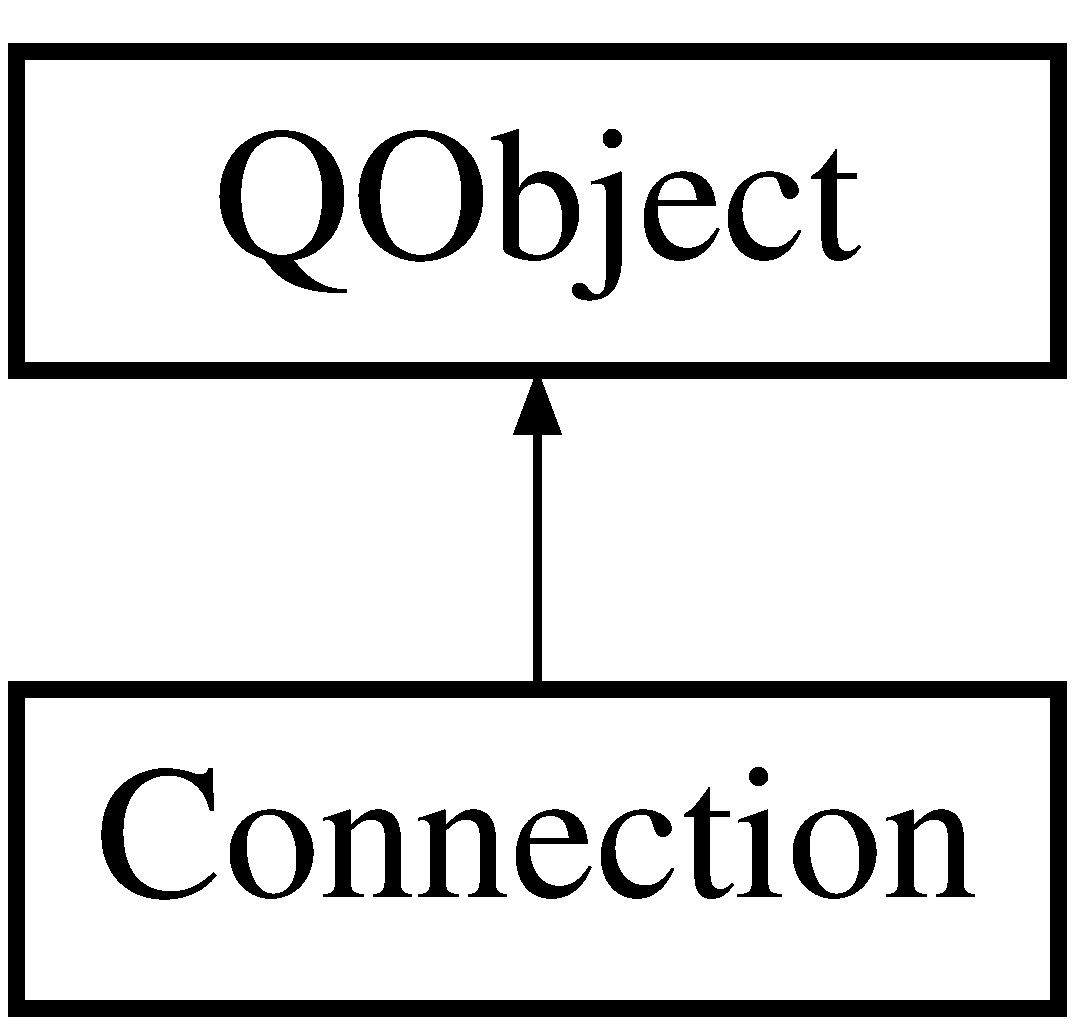
\includegraphics[height=2.000000cm]{classConnection}
\end{center}
\end{figure}
\subsection*{Signals}
\begin{DoxyCompactItemize}
\item 
\mbox{\Hypertarget{classConnection_a33165f69da60f638d3d8412e3ccc4312}\label{classConnection_a33165f69da60f638d3d8412e3ccc4312}} 
void {\bfseries receiver\+Changed} ()
\item 
\mbox{\Hypertarget{classConnection_acd694eeb6ad7e287aacd356b95fe6dd9}\label{classConnection_acd694eeb6ad7e287aacd356b95fe6dd9}} 
void {\bfseries sender\+Changed} ()
\end{DoxyCompactItemize}
\subsection*{Public Member Functions}
\begin{DoxyCompactItemize}
\item 
\mbox{\Hypertarget{classConnection_a8afe63c8ac9873d6e01e2ca19218344e}\label{classConnection_a8afe63c8ac9873d6e01e2ca19218344e}} 
{\bfseries Connection} (Q\+Object $\ast$parent=nullptr)
\item 
\mbox{\Hypertarget{classConnection_ab510cb0a3cf64e4d98f624e73728bec0}\label{classConnection_ab510cb0a3cf64e4d98f624e73728bec0}} 
\mbox{\hyperlink{classNode}{Node}} $\ast$ {\bfseries receiver} () const
\item 
\mbox{\Hypertarget{classConnection_af28434b67e1e6c6930f5363612dda233}\label{classConnection_af28434b67e1e6c6930f5363612dda233}} 
\mbox{\hyperlink{classNode}{Node}} $\ast$ {\bfseries sender} () const
\item 
\mbox{\Hypertarget{classConnection_ac7e9230266e557439f1597d14d92bd41}\label{classConnection_ac7e9230266e557439f1597d14d92bd41}} 
void {\bfseries set\+Receiver} (\mbox{\hyperlink{classNode}{Node}} $\ast$n)
\item 
\mbox{\Hypertarget{classConnection_aab3e0207b72d5af2dfbf6c0757ecc4da}\label{classConnection_aab3e0207b72d5af2dfbf6c0757ecc4da}} 
void {\bfseries set\+Sender} (\mbox{\hyperlink{classNode}{Node}} $\ast$n)
\item 
\mbox{\Hypertarget{classConnection_ad75ed4e7c64886d0a7b1b229da1087a6}\label{classConnection_ad75ed4e7c64886d0a7b1b229da1087a6}} 
void {\bfseries read} (const Q\+Json\+Object \&json, const Q\+Hash$<$ qulonglong, \mbox{\hyperlink{classNode}{Node}} $\ast$$>$ \&hash)
\item 
\mbox{\Hypertarget{classConnection_a8e141967a494f7e3d577fe018cfa5178}\label{classConnection_a8e141967a494f7e3d577fe018cfa5178}} 
Q\+Json\+Object {\bfseries write} () const
\end{DoxyCompactItemize}
\subsection*{Properties}
\begin{DoxyCompactItemize}
\item 
\mbox{\Hypertarget{classConnection_a801ac88d7985062c01ebff75ca3845a7}\label{classConnection_a801ac88d7985062c01ebff75ca3845a7}} 
\mbox{\hyperlink{classNode}{Node}} {\bfseries to}
\item 
\mbox{\Hypertarget{classConnection_a9e0992b9aebf3307aa05ef797ed8426d}\label{classConnection_a9e0992b9aebf3307aa05ef797ed8426d}} 
\mbox{\hyperlink{classNode}{Node}} {\bfseries from}
\end{DoxyCompactItemize}
\subsection*{Private Attributes}
\begin{DoxyCompactItemize}
\item 
\mbox{\Hypertarget{classConnection_a508ae4ca471baad98e9ace730e8ab500}\label{classConnection_a508ae4ca471baad98e9ace730e8ab500}} 
\mbox{\hyperlink{classNode}{Node}} $\ast$ {\bfseries m\+\_\+receiver}
\item 
\mbox{\Hypertarget{classConnection_aa6eb9bca71cf1144595325a4c47182b9}\label{classConnection_aa6eb9bca71cf1144595325a4c47182b9}} 
\mbox{\hyperlink{classNode}{Node}} $\ast$ {\bfseries m\+\_\+sender}
\end{DoxyCompactItemize}


The documentation for this class was generated from the following files\+:\begin{DoxyCompactItemize}
\item 
include/connection.\+h\item 
src/cpp/connection.\+cpp\end{DoxyCompactItemize}

\hypertarget{classNode}{}\section{Node Class Reference}
\label{classNode}\index{Node@{Node}}
Inheritance diagram for Node\+:\begin{figure}[H]
\begin{center}
\leavevmode
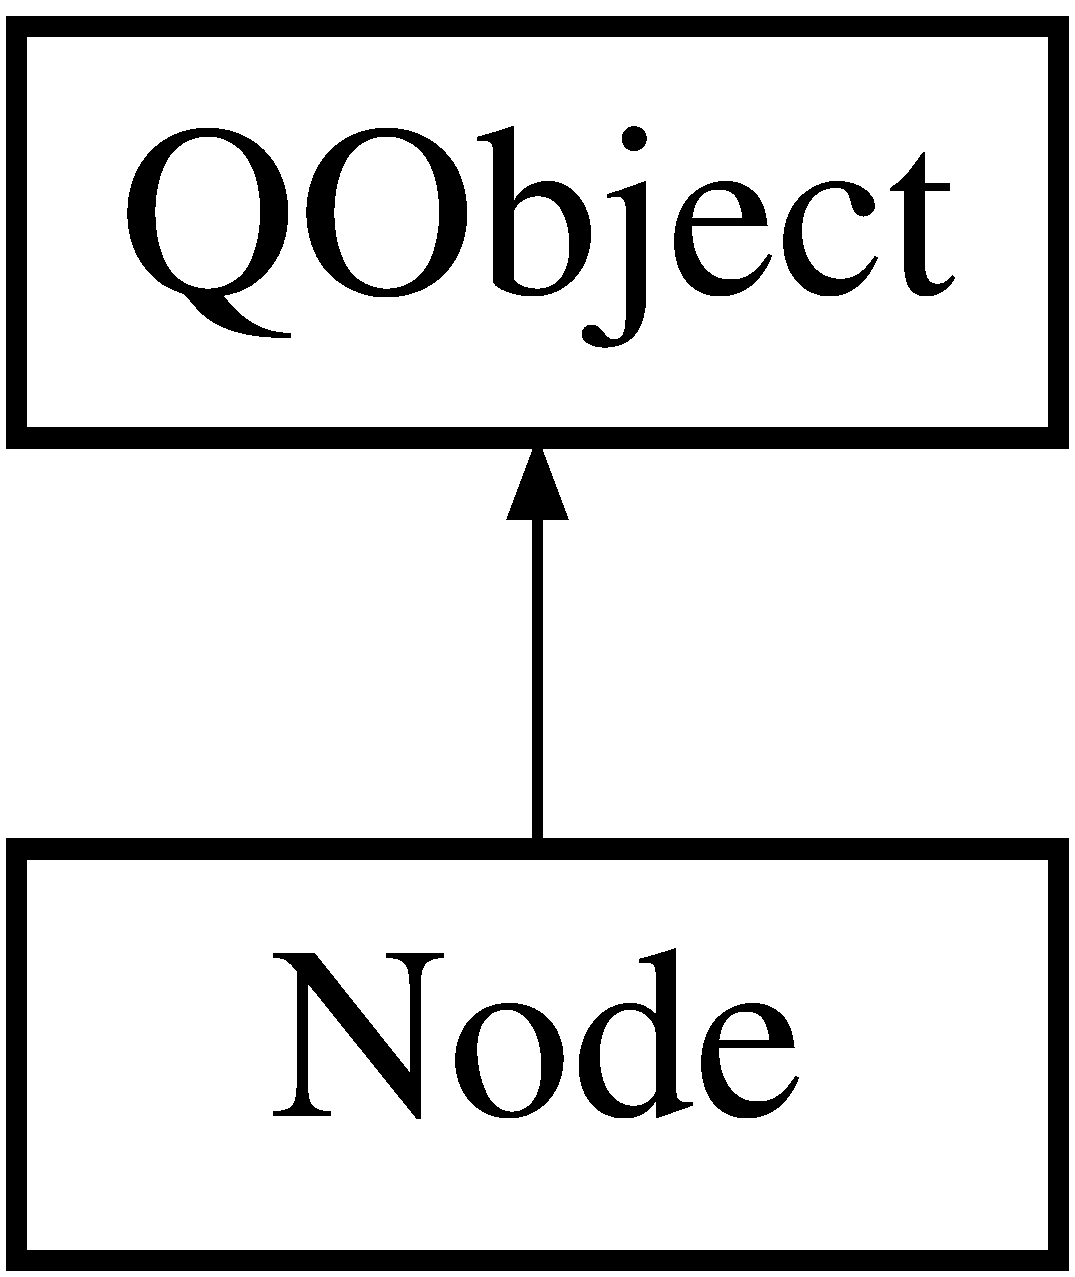
\includegraphics[height=2.000000cm]{classNode}
\end{center}
\end{figure}
\subsection*{Public Types}
\begin{DoxyCompactItemize}
\item 
\mbox{\Hypertarget{classNode_a8dad370be1595f49e0a7c2406a91e867}\label{classNode_a8dad370be1595f49e0a7c2406a91e867}} 
enum {\bfseries Type} \{ \newline
{\bfseries Input} = 0, 
\newline
{\bfseries Output} = 1, 
\newline
{\bfseries Or\+Gate} = 10, 
\newline
{\bfseries And\+Gate} = 11
 \}
\end{DoxyCompactItemize}
\subsection*{Signals}
\begin{DoxyCompactItemize}
\item 
\mbox{\Hypertarget{classNode_adcbfe89009445eca17b8d9e122c504f4}\label{classNode_adcbfe89009445eca17b8d9e122c504f4}} 
void {\bfseries type\+Changed} ()
\item 
\mbox{\Hypertarget{classNode_ab1a77a5a5faea93bbf412647885688f9}\label{classNode_ab1a77a5a5faea93bbf412647885688f9}} 
void {\bfseries name\+Changed} ()
\item 
\mbox{\Hypertarget{classNode_aacc34a3cf4a311bf9d655c8b90098f6a}\label{classNode_aacc34a3cf4a311bf9d655c8b90098f6a}} 
void {\bfseries address\+Changed} ()
\item 
\mbox{\Hypertarget{classNode_ae985827a18c3c371a4979e93fd18f6a6}\label{classNode_ae985827a18c3c371a4979e93fd18f6a6}} 
void {\bfseries ip\+Changed} ()
\item 
\mbox{\Hypertarget{classNode_a8454690655da62155f182fcc1e523bfb}\label{classNode_a8454690655da62155f182fcc1e523bfb}} 
void {\bfseries connections\+Have\+Changed} ()
\item 
\mbox{\Hypertarget{classNode_a7ef0676f32b351a179a0ef09491b7dbd}\label{classNode_a7ef0676f32b351a179a0ef09491b7dbd}} 
void {\bfseries pos\+Changed} ()
\item 
\mbox{\Hypertarget{classNode_a71aeb141261b0cacb7e4562f9d3e3584}\label{classNode_a71aeb141261b0cacb7e4562f9d3e3584}} 
void {\bfseries in\+Pos\+Changed} ()
\item 
\mbox{\Hypertarget{classNode_a672f3bac02b8d931dbc70221bcec5f82}\label{classNode_a672f3bac02b8d931dbc70221bcec5f82}} 
void {\bfseries out\+Pos\+Changed} ()
\item 
\mbox{\Hypertarget{classNode_a9d5d3ed653b8334849f3c0738dc6000e}\label{classNode_a9d5d3ed653b8334849f3c0738dc6000e}} 
void {\bfseries output\+Changed} ()
\item 
\mbox{\Hypertarget{classNode_a64a8638185a74040be7526961bf60dca}\label{classNode_a64a8638185a74040be7526961bf60dca}} 
void {\bfseries bound\+Changed} ()
\item 
\mbox{\Hypertarget{classNode_a9e9cd320a947a1d2ee154430295a5081}\label{classNode_a9e9cd320a947a1d2ee154430295a5081}} 
void {\bfseries opened\+Changed} ()
\item 
\mbox{\Hypertarget{classNode_a03a32d400001bc8871a6bd5f31c70b19}\label{classNode_a03a32d400001bc8871a6bd5f31c70b19}} 
void {\bfseries inverted\+Changed} ()
\item 
\mbox{\Hypertarget{classNode_a1f66a3111cc14cd1fc8ca4db3741429b}\label{classNode_a1f66a3111cc14cd1fc8ca4db3741429b}} 
void {\bfseries message\+Ready} (\mbox{\hyperlink{classNode}{Node}} $\ast$)
\item 
\mbox{\Hypertarget{classNode_a3644e5a194e3f4d83860cd7118d49fe3}\label{classNode_a3644e5a194e3f4d83860cd7118d49fe3}} 
void {\bfseries value\+Changed} ()
\item 
\mbox{\Hypertarget{classNode_a0110e86c6ae22ba29fc5660d142416d1}\label{classNode_a0110e86c6ae22ba29fc5660d142416d1}} 
void {\bfseries node\+Have\+Changed} ()
\item 
\mbox{\Hypertarget{classNode_a9ae68ff6254a48d2d11f72161fecf67e}\label{classNode_a9ae68ff6254a48d2d11f72161fecf67e}} 
void {\bfseries min\+Changed} ()
\item 
\mbox{\Hypertarget{classNode_ab05844c4ab39602e886f19c72cc49763}\label{classNode_ab05844c4ab39602e886f19c72cc49763}} 
void {\bfseries max\+Changed} ()
\item 
\mbox{\Hypertarget{classNode_a5fec832ac372cd32eb5724cdac8be048}\label{classNode_a5fec832ac372cd32eb5724cdac8be048}} 
void {\bfseries first\+Changed} ()
\item 
\mbox{\Hypertarget{classNode_ae62835ad14946daf008cdd2887e2af8c}\label{classNode_ae62835ad14946daf008cdd2887e2af8c}} 
void {\bfseries second\+Changed} ()
\item 
\mbox{\Hypertarget{classNode_a457f927fed0506072d24960cc69a8c58}\label{classNode_a457f927fed0506072d24960cc69a8c58}} 
void {\bfseries method\+Changed} ()
\item 
\mbox{\Hypertarget{classNode_a25cfd54debef015217a521dabfcb9f79}\label{classNode_a25cfd54debef015217a521dabfcb9f79}} 
void {\bfseries condition\+Overriden} ()
\end{DoxyCompactItemize}
\subsection*{Public Member Functions}
\begin{DoxyCompactItemize}
\item 
\mbox{\Hypertarget{classNode_a96f101eb67925097d69051a242b8e5a7}\label{classNode_a96f101eb67925097d69051a242b8e5a7}} 
{\bfseries Node} (Q\+Object $\ast$parent=nullptr)
\item 
\mbox{\Hypertarget{classNode_a16da82741d426eed77c481ab13a2fb7c}\label{classNode_a16da82741d426eed77c481ab13a2fb7c}} 
Q\+Point {\bfseries pos} () const
\item 
\mbox{\Hypertarget{classNode_a31619f2d1580d4c97d1c454c04a3ce7e}\label{classNode_a31619f2d1580d4c97d1c454c04a3ce7e}} 
void {\bfseries set\+Pos} (const Q\+Point \&p)
\item 
\mbox{\Hypertarget{classNode_a7f2ad8fdb2afa9c0369c35a2270d93f1}\label{classNode_a7f2ad8fdb2afa9c0369c35a2270d93f1}} 
Q\+Point {\bfseries in\+Pos} () const
\item 
\mbox{\Hypertarget{classNode_aa34d51c11117d2e01e707f84d7c5c2a0}\label{classNode_aa34d51c11117d2e01e707f84d7c5c2a0}} 
void {\bfseries set\+In\+Pos} (const Q\+Point \&p)
\item 
\mbox{\Hypertarget{classNode_a1caba8cbccfaf15e73ffe620e3e293fc}\label{classNode_a1caba8cbccfaf15e73ffe620e3e293fc}} 
Q\+Point {\bfseries out\+Pos} () const
\item 
\mbox{\Hypertarget{classNode_aa5db2e2bc6aef41e31f1977d9b487c1c}\label{classNode_aa5db2e2bc6aef41e31f1977d9b487c1c}} 
void {\bfseries set\+Out\+Pos} (const Q\+Point \&p)
\item 
\mbox{\Hypertarget{classNode_a347703417d88a057b631fb88e6251fe7}\label{classNode_a347703417d88a057b631fb88e6251fe7}} 
void {\bfseries set\+Type} (const Type \&t)
\item 
\mbox{\Hypertarget{classNode_a2cd393eb2422071ed2af7e026e61c7cb}\label{classNode_a2cd393eb2422071ed2af7e026e61c7cb}} 
Type {\bfseries type} () const
\item 
\mbox{\Hypertarget{classNode_a05a2a996157abda66ef7da3baf2f5db3}\label{classNode_a05a2a996157abda66ef7da3baf2f5db3}} 
void {\bfseries set\+Value} (const double \&v)
\item 
\mbox{\Hypertarget{classNode_a508e7ab9a2c9feed1ab311606e9e1b68}\label{classNode_a508e7ab9a2c9feed1ab311606e9e1b68}} 
double {\bfseries value} () const
\item 
\mbox{\Hypertarget{classNode_a8c58d22a60a161c24f5668be303a11c5}\label{classNode_a8c58d22a60a161c24f5668be303a11c5}} 
void {\bfseries set\+Name} (const Q\+String \&n)
\item 
\mbox{\Hypertarget{classNode_ac40f16db9ad108a3d8a029802899104c}\label{classNode_ac40f16db9ad108a3d8a029802899104c}} 
Q\+String {\bfseries name} () const
\item 
\mbox{\Hypertarget{classNode_a501c58ee4e1197e670459a80ccc121f7}\label{classNode_a501c58ee4e1197e670459a80ccc121f7}} 
void {\bfseries set\+Address} (const Q\+String \&i)
\item 
\mbox{\Hypertarget{classNode_a51460cca215d98243c8efd817713b7e3}\label{classNode_a51460cca215d98243c8efd817713b7e3}} 
Q\+String {\bfseries address} () const
\item 
\mbox{\Hypertarget{classNode_a1141569603eaccd819188c5dbfa9a9f9}\label{classNode_a1141569603eaccd819188c5dbfa9a9f9}} 
void {\bfseries set\+Output} (const bool \&o)
\item 
\mbox{\Hypertarget{classNode_a8c4ed49f3a1033f0ebd945170e780231}\label{classNode_a8c4ed49f3a1033f0ebd945170e780231}} 
bool {\bfseries output} () const
\item 
\mbox{\Hypertarget{classNode_ac0827ecef276b83a1b24306f69258ca4}\label{classNode_ac0827ecef276b83a1b24306f69258ca4}} 
void {\bfseries set\+Bound} (const bool \&i)
\item 
\mbox{\Hypertarget{classNode_a9540c4684a7d3d94d08ea673762488b5}\label{classNode_a9540c4684a7d3d94d08ea673762488b5}} 
bool {\bfseries bound} () const
\item 
\mbox{\Hypertarget{classNode_ae6c46260f6887d83837ed895cc24c9c4}\label{classNode_ae6c46260f6887d83837ed895cc24c9c4}} 
void {\bfseries set\+Opened} (const bool \&o)
\item 
\mbox{\Hypertarget{classNode_abe055b7d4469fcce0b3550a2096ab256}\label{classNode_abe055b7d4469fcce0b3550a2096ab256}} 
bool {\bfseries opened} () const
\item 
\mbox{\Hypertarget{classNode_a75733c30a1b1f73e439e6030702bc516}\label{classNode_a75733c30a1b1f73e439e6030702bc516}} 
void {\bfseries set\+Inverted} (const bool \&i)
\item 
\mbox{\Hypertarget{classNode_a1f3f2f1e2a3d58b480a9896d14c925ed}\label{classNode_a1f3f2f1e2a3d58b480a9896d14c925ed}} 
bool {\bfseries inverted} () const
\item 
\mbox{\Hypertarget{classNode_a9281d0e024c9dba7e3ce4ac7f0929a09}\label{classNode_a9281d0e024c9dba7e3ce4ac7f0929a09}} 
void {\bfseries set\+Min} (const double \&rs)
\item 
\mbox{\Hypertarget{classNode_ab3916a71937c0f290096ba5ceb83e446}\label{classNode_ab3916a71937c0f290096ba5ceb83e446}} 
double {\bfseries min} () const
\item 
\mbox{\Hypertarget{classNode_a4f72734abbd068beab2bb5efa325239d}\label{classNode_a4f72734abbd068beab2bb5efa325239d}} 
void {\bfseries set\+Max} (const double \&re)
\item 
\mbox{\Hypertarget{classNode_a5e3869dd6d197f443d15aedec21653a4}\label{classNode_a5e3869dd6d197f443d15aedec21653a4}} 
double {\bfseries max} () const
\item 
\mbox{\Hypertarget{classNode_a95b19867e7793bd169a5338f109656b1}\label{classNode_a95b19867e7793bd169a5338f109656b1}} 
void {\bfseries set\+First} (const double \&rm)
\item 
\mbox{\Hypertarget{classNode_ada611ffb36ad9b6cadc81a8287c6d10f}\label{classNode_ada611ffb36ad9b6cadc81a8287c6d10f}} 
double {\bfseries first} () const
\item 
\mbox{\Hypertarget{classNode_ae39defb336f6881f50fce60e88ce76be}\label{classNode_ae39defb336f6881f50fce60e88ce76be}} 
void {\bfseries set\+Second} (const double \&rm)
\item 
\mbox{\Hypertarget{classNode_a6c71292db71aac8c9742f13583f915ad}\label{classNode_a6c71292db71aac8c9742f13583f915ad}} 
double {\bfseries second} () const
\item 
\mbox{\Hypertarget{classNode_a2222f4650793659e8579c2eb725f029d}\label{classNode_a2222f4650793659e8579c2eb725f029d}} 
void {\bfseries set\+Ip} (const Q\+String \&i)
\item 
\mbox{\Hypertarget{classNode_a42fea6791a936f0255c5a8207e6a778e}\label{classNode_a42fea6791a936f0255c5a8207e6a778e}} 
Q\+String {\bfseries ip} () const
\item 
\mbox{\Hypertarget{classNode_a4479a7c2e0f48ed75133ca45b42ad339}\label{classNode_a4479a7c2e0f48ed75133ca45b42ad339}} 
Q\+Host\+Address {\bfseries get\+Ip} () const
\item 
\mbox{\Hypertarget{classNode_a114811570f6e6b2711635747af138e68}\label{classNode_a114811570f6e6b2711635747af138e68}} 
quint16 {\bfseries get\+Port} () const
\item 
\mbox{\Hypertarget{classNode_a8f3da5e81c2e206943236b3bf77589a1}\label{classNode_a8f3da5e81c2e206943236b3bf77589a1}} 
qulonglong {\bfseries id} () const
\item 
\mbox{\Hypertarget{classNode_abcfc7dbcab27b9ffd29830b599337529}\label{classNode_abcfc7dbcab27b9ffd29830b599337529}} 
void {\bfseries read} (const Q\+Json\+Object \&json)
\item 
\mbox{\Hypertarget{classNode_a30c4929b3a320cdab5e4e7e60126de5c}\label{classNode_a30c4929b3a320cdab5e4e7e60126de5c}} 
Q\+Json\+Object {\bfseries write} () const
\item 
\mbox{\Hypertarget{classNode_a86f94f425dbee2eff2e43c22f5a2dc45}\label{classNode_a86f94f425dbee2eff2e43c22f5a2dc45}} 
Q\+Point {\bfseries read\+Point} (const Q\+Json\+Object \&) const
\item 
\mbox{\Hypertarget{classNode_adfa903ce53347a33484770e92787fb37}\label{classNode_adfa903ce53347a33484770e92787fb37}} 
Q\+Json\+Object {\bfseries write\+Point} (const Q\+Point \&) const
\end{DoxyCompactItemize}
\subsection*{Properties}
\begin{DoxyCompactItemize}
\item 
\mbox{\Hypertarget{classNode_a2d594c1fd5e6bb196ac972950b3b003f}\label{classNode_a2d594c1fd5e6bb196ac972950b3b003f}} 
Type {\bfseries type}
\item 
\mbox{\Hypertarget{classNode_a91f9e234953a33d2bd876a7a748c85ec}\label{classNode_a91f9e234953a33d2bd876a7a748c85ec}} 
double {\bfseries value}
\item 
\mbox{\Hypertarget{classNode_a4eb46a970b73d2edf10cb289f3df8e01}\label{classNode_a4eb46a970b73d2edf10cb289f3df8e01}} 
bool {\bfseries output}
\item 
\mbox{\Hypertarget{classNode_ad864ab24f394b18f2ed1fdb56b3340eb}\label{classNode_ad864ab24f394b18f2ed1fdb56b3340eb}} 
Q\+String {\bfseries name}
\item 
\mbox{\Hypertarget{classNode_af5b57623b505b9471206ddd8e25831e9}\label{classNode_af5b57623b505b9471206ddd8e25831e9}} 
Q\+String {\bfseries address}
\item 
\mbox{\Hypertarget{classNode_ad9404669683d5d12c819c646753d9428}\label{classNode_ad9404669683d5d12c819c646753d9428}} 
Q\+String {\bfseries ip}
\item 
\mbox{\Hypertarget{classNode_a36ff894ab042668791da153b7141e6de}\label{classNode_a36ff894ab042668791da153b7141e6de}} 
bool {\bfseries bound}
\item 
\mbox{\Hypertarget{classNode_a0ec5043d06a7b57d2649d9a7b4f85643}\label{classNode_a0ec5043d06a7b57d2649d9a7b4f85643}} 
bool {\bfseries opened}
\item 
\mbox{\Hypertarget{classNode_a4f9c4c86f80c90e5082df3f9bb5c8d40}\label{classNode_a4f9c4c86f80c90e5082df3f9bb5c8d40}} 
bool {\bfseries inverted}
\item 
\mbox{\Hypertarget{classNode_a17543f5c5b9eaf3cb47317d9abc2e1d2}\label{classNode_a17543f5c5b9eaf3cb47317d9abc2e1d2}} 
Q\+Point {\bfseries pos}
\item 
\mbox{\Hypertarget{classNode_a94d763fca0bb262a443eb8954c29cca3}\label{classNode_a94d763fca0bb262a443eb8954c29cca3}} 
Q\+Point {\bfseries in\+Pos}
\item 
\mbox{\Hypertarget{classNode_a68f8844b5a417d24a73c5a42053f7b83}\label{classNode_a68f8844b5a417d24a73c5a42053f7b83}} 
Q\+Point {\bfseries out\+Pos}
\item 
\mbox{\Hypertarget{classNode_a13a0780efbfb45fa05f71db05101d0b5}\label{classNode_a13a0780efbfb45fa05f71db05101d0b5}} 
double {\bfseries min}
\item 
\mbox{\Hypertarget{classNode_a12dde336ea8459ddb531efcdd0efccae}\label{classNode_a12dde336ea8459ddb531efcdd0efccae}} 
double {\bfseries max}
\item 
\mbox{\Hypertarget{classNode_a649bdd5c69dfb539bc129d2c074f03ea}\label{classNode_a649bdd5c69dfb539bc129d2c074f03ea}} 
double {\bfseries first}
\item 
\mbox{\Hypertarget{classNode_a4fb62aa24764bae14627d3afc4039572}\label{classNode_a4fb62aa24764bae14627d3afc4039572}} 
double {\bfseries second}
\end{DoxyCompactItemize}
\subsection*{Private Attributes}
\begin{DoxyCompactItemize}
\item 
\mbox{\Hypertarget{classNode_a212e46e3de8f152be26c55810f504bd0}\label{classNode_a212e46e3de8f152be26c55810f504bd0}} 
Q\+String {\bfseries m\+\_\+name} = \char`\"{}Name\char`\"{}
\item 
\mbox{\Hypertarget{classNode_a229782743d15a6963d87ba406bac67c4}\label{classNode_a229782743d15a6963d87ba406bac67c4}} 
Q\+String {\bfseries m\+\_\+address} = \char`\"{}/home/default\char`\"{}
\item 
\mbox{\Hypertarget{classNode_a9eef6ea1453c387e542e23e85a571fdf}\label{classNode_a9eef6ea1453c387e542e23e85a571fdf}} 
Q\+String {\bfseries m\+\_\+ip} = \char`\"{}127.\+0.\+0.\+1\+:8888\char`\"{}
\item 
\mbox{\Hypertarget{classNode_a43c294b967c1b5a6b73060d51824aa4d}\label{classNode_a43c294b967c1b5a6b73060d51824aa4d}} 
Q\+Point {\bfseries m\+\_\+pos}
\item 
\mbox{\Hypertarget{classNode_a8dc9a65d78186e49bbc5fe817b1104f2}\label{classNode_a8dc9a65d78186e49bbc5fe817b1104f2}} 
Q\+Point {\bfseries m\+\_\+in}
\item 
\mbox{\Hypertarget{classNode_ab8f3fbda818d7454fa5cb34e078418f3}\label{classNode_ab8f3fbda818d7454fa5cb34e078418f3}} 
Q\+Point {\bfseries m\+\_\+out}
\item 
\mbox{\Hypertarget{classNode_a82da945ee34133f197fd8dcefc9070a0}\label{classNode_a82da945ee34133f197fd8dcefc9070a0}} 
Type {\bfseries m\+\_\+type} = Node\+::\+Input
\item 
\mbox{\Hypertarget{classNode_a7dc02eca908f23a9bf1286d64e9d85c6}\label{classNode_a7dc02eca908f23a9bf1286d64e9d85c6}} 
double {\bfseries m\+\_\+value} = 0.\+0
\item 
\mbox{\Hypertarget{classNode_a6c5c7957cd96ee186cd172f0ca160cff}\label{classNode_a6c5c7957cd96ee186cd172f0ca160cff}} 
double {\bfseries m\+\_\+min} = 0.\+0
\item 
\mbox{\Hypertarget{classNode_a989f95ea5a316010c4e10f8f4b9dda9f}\label{classNode_a989f95ea5a316010c4e10f8f4b9dda9f}} 
double {\bfseries m\+\_\+max} = 100.\+0
\item 
\mbox{\Hypertarget{classNode_ab7660bde372ab02cedcbb810ed878216}\label{classNode_ab7660bde372ab02cedcbb810ed878216}} 
double {\bfseries m\+\_\+first} = 25.\+0
\item 
\mbox{\Hypertarget{classNode_a9a2c75b4e1cc47bb465b6e032d6aa11e}\label{classNode_a9a2c75b4e1cc47bb465b6e032d6aa11e}} 
double {\bfseries m\+\_\+second} = 75.\+0
\item 
\mbox{\Hypertarget{classNode_a5c0e1404f737864c62e810fe595c7bde}\label{classNode_a5c0e1404f737864c62e810fe595c7bde}} 
bool {\bfseries m\+\_\+output} = true
\item 
\mbox{\Hypertarget{classNode_aad787043f0df6d527c391ea50583250a}\label{classNode_aad787043f0df6d527c391ea50583250a}} 
bool {\bfseries m\+\_\+bound} = false
\item 
\mbox{\Hypertarget{classNode_adb24661af93e1a2749cf360191781d5f}\label{classNode_adb24661af93e1a2749cf360191781d5f}} 
bool {\bfseries m\+\_\+opened} = true
\item 
\mbox{\Hypertarget{classNode_af1127c01cdf01117e053022ab8777768}\label{classNode_af1127c01cdf01117e053022ab8777768}} 
bool {\bfseries m\+\_\+inverted} = false
\item 
\mbox{\Hypertarget{classNode_a5c1c0ff28c4d71f57d44400cba820caa}\label{classNode_a5c1c0ff28c4d71f57d44400cba820caa}} 
qulonglong {\bfseries m\+\_\+id}
\end{DoxyCompactItemize}


The documentation for this class was generated from the following files\+:\begin{DoxyCompactItemize}
\item 
include/node.\+h\item 
src/cpp/node.\+cpp\end{DoxyCompactItemize}

\hypertarget{classRoom}{}\section{Room Class Reference}
\label{classRoom}\index{Room@{Room}}


Backend class representing a room.  




{\ttfamily \#include $<$room.\+h$>$}

Inheritance diagram for Room\+:\begin{figure}[H]
\begin{center}
\leavevmode
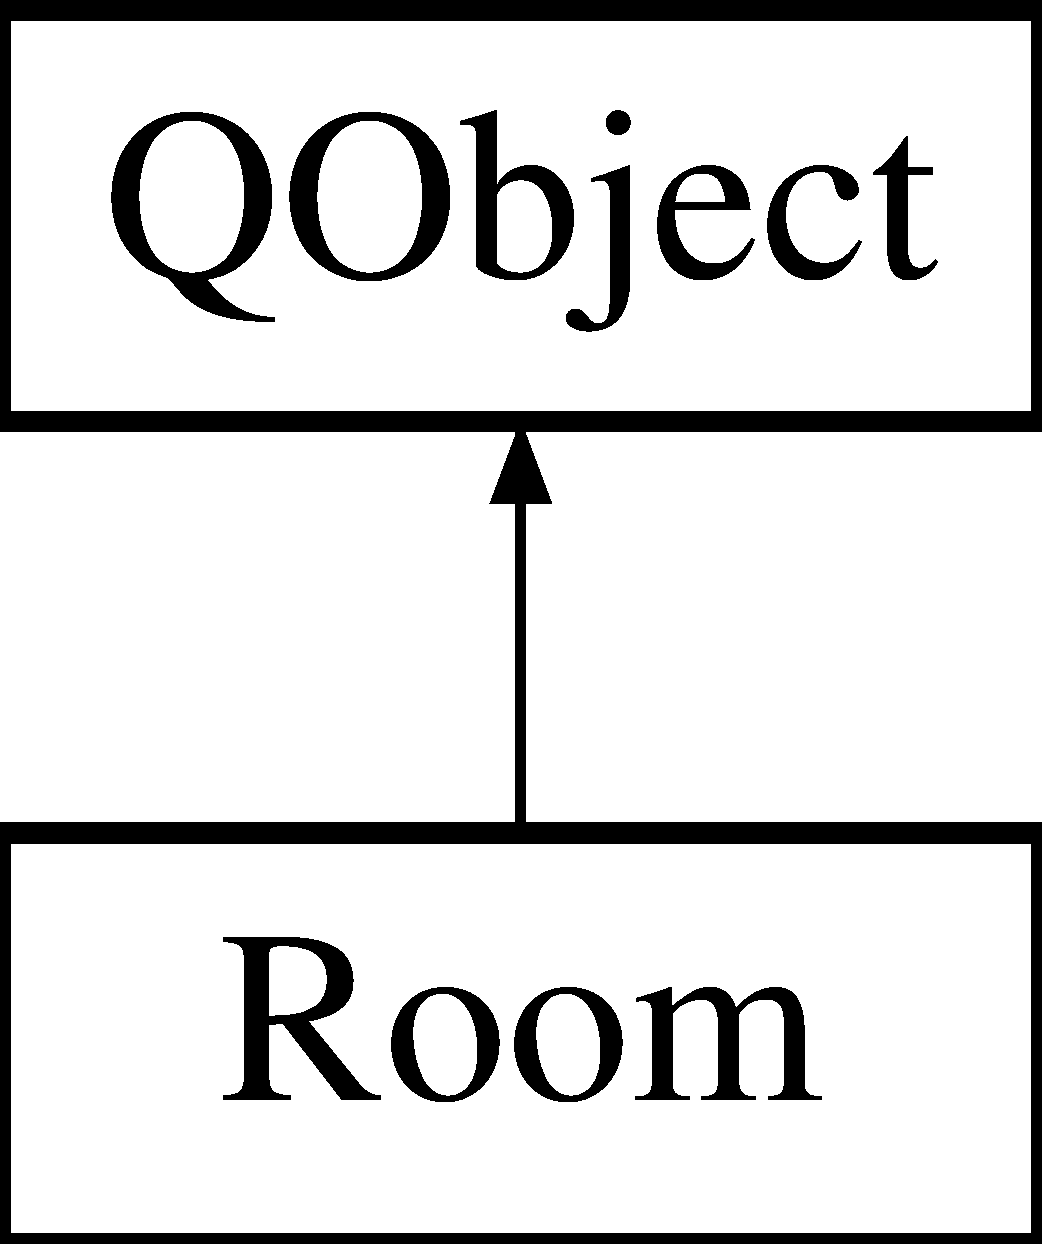
\includegraphics[height=2.000000cm]{classRoom}
\end{center}
\end{figure}
\subsection*{Signals}
\begin{DoxyCompactItemize}
\item 
void \mbox{\hyperlink{classRoom_a4fad3e109783442157bb775ef417a57b}{connections\+Updated}} ()
\item 
void \mbox{\hyperlink{classRoom_a8261085c6843f3b85d403284b39f92ba}{nodes\+Updated}} ()
\item 
void \mbox{\hyperlink{classRoom_abc28a6555cb3e3543eecb65095ee89b7}{file\+Changed}} ()
\item 
void \mbox{\hyperlink{classRoom_ae37847fde9763f0561150f8bcfa0b550}{room\+Have\+Changed}} ()
\item 
void \mbox{\hyperlink{classRoom_abe1f81891e69cd6b511bbf18d7ce38c2}{room\+Loaded}} ()
\end{DoxyCompactItemize}
\subsection*{Public Member Functions}
\begin{DoxyCompactItemize}
\item 
\mbox{\hyperlink{classRoom_a58d54cc7a80930812d780f101c1dc4bc}{Room}} (Q\+Object $\ast$parent=nullptr)
\begin{DoxyCompactList}\small\item\em Default constructor. \end{DoxyCompactList}\item 
Q\+Qml\+List\+Property$<$ \mbox{\hyperlink{classConnection}{Connection}} $>$ \mbox{\hyperlink{classRoom_a95230e582f089891ea8a8f6febfaf2fa}{connections}} ()
\begin{DoxyCompactList}\small\item\em Getter method to expose the list of connections to Q\+ML. \end{DoxyCompactList}\item 
Q\+Qml\+List\+Property$<$ \mbox{\hyperlink{classNode}{Node}} $>$ \mbox{\hyperlink{classRoom_a9ed01ab71422acf2c22b46d7f582f878}{nodes}} ()
\begin{DoxyCompactList}\small\item\em Getter method to expose the list of nodes to Q\+ML. \end{DoxyCompactList}\item 
Q\+Url \mbox{\hyperlink{classRoom_ab6644a3874458fbeffd5fa2951d281ab}{file}} () const
\begin{DoxyCompactList}\small\item\em Getter method to expose the file used for saving to Q\+ML. \end{DoxyCompactList}\item 
void \mbox{\hyperlink{classRoom_afe61f8f1359a431ef906ee2ff485eb80}{set\+File}} (const Q\+Url \&url)
\begin{DoxyCompactList}\small\item\em Setter to change the file in which changes are to be saved. \end{DoxyCompactList}\item 
Q\+\_\+\+I\+N\+V\+O\+K\+A\+B\+LE bool \mbox{\hyperlink{classRoom_adbcc976eefed696d0536773e75c4f7d2}{delete\+Node}} (\mbox{\hyperlink{classNode}{Node}} $\ast$node)
\begin{DoxyCompactList}\small\item\em Q\+ML exposed method to remove nodes from the room. \end{DoxyCompactList}\item 
Q\+\_\+\+I\+N\+V\+O\+K\+A\+B\+LE bool \mbox{\hyperlink{classRoom_aaaeb040b9fa13894f4c19fb1eecbefd2}{connected}} (\mbox{\hyperlink{classNode}{Node}} $\ast$a, \mbox{\hyperlink{classNode}{Node}} $\ast$b, int direction=Node\+::\+Input)
\begin{DoxyCompactList}\small\item\em Checks if two nodes are connected in a certain direction. \end{DoxyCompactList}\item 
Q\+\_\+\+I\+N\+V\+O\+K\+A\+B\+LE bool \mbox{\hyperlink{classRoom_a085e1c1c95f6d30dded1ace857a3ec09}{can\+Connect}} (\mbox{\hyperlink{classNode}{Node}} $\ast$a, \mbox{\hyperlink{classNode}{Node}} $\ast$b, int direction=Node\+::\+Input)
\begin{DoxyCompactList}\small\item\em Checks all conditions before connecting two nodes. \end{DoxyCompactList}\item 
Q\+\_\+\+I\+N\+V\+O\+K\+A\+B\+LE void \mbox{\hyperlink{classRoom_a0b0b13f4ebd1c45353090b6ac64ed433}{remove\+Connections}} (\mbox{\hyperlink{classNode}{Node}} $\ast$a, \mbox{\hyperlink{classNode}{Node}} $\ast$b, int t=Node\+::\+Input)
\begin{DoxyCompactList}\small\item\em Breaks any connections between two nodes in a certain direction. \end{DoxyCompactList}\item 
Q\+\_\+\+I\+N\+V\+O\+K\+A\+B\+LE void \mbox{\hyperlink{classRoom_a3a88ea31e062677f1d245960b20a6e97}{create\+Connection}} (\mbox{\hyperlink{classNode}{Node}} $\ast$a, \mbox{\hyperlink{classNode}{Node}} $\ast$b, int t=Node\+::\+Input)
\begin{DoxyCompactList}\small\item\em Establish a connection between two nodes in a certain direction. \end{DoxyCompactList}\item 
Q\+\_\+\+I\+N\+V\+O\+K\+A\+B\+LE bool \mbox{\hyperlink{classRoom_ad942f0c7132818f36a4de16fe2ca477a}{has\+Out\+Connection}} (\mbox{\hyperlink{classNode}{Node}} $\ast$node)
\begin{DoxyCompactList}\small\item\em Check if a node is the sender in any connection in the room. \end{DoxyCompactList}\item 
Q\+\_\+\+I\+N\+V\+O\+K\+A\+B\+LE bool \mbox{\hyperlink{classRoom_aeffeac1d449a9a713efcf94efb2432e0}{has\+In\+Connection}} (\mbox{\hyperlink{classNode}{Node}} $\ast$node)
\begin{DoxyCompactList}\small\item\em Check if a node is the receiver in any connection in the room. \end{DoxyCompactList}\item 
Q\+\_\+\+I\+N\+V\+O\+K\+A\+B\+LE void \mbox{\hyperlink{classRoom_a0f8b282b43bd3115e24f6b9bd95d92a9}{evaluate}} (\mbox{\hyperlink{classNode}{Node}} $\ast$node)
\begin{DoxyCompactList}\small\item\em Change the output value of a node based on connections and the nodes\textquotesingle{} configuration. \end{DoxyCompactList}\item 
\mbox{\Hypertarget{classRoom_a4d01284c86cb970b25b0fcfa45cdd38e}\label{classRoom_a4d01284c86cb970b25b0fcfa45cdd38e}} 
Q\+\_\+\+I\+N\+V\+O\+K\+A\+B\+LE void \mbox{\hyperlink{classRoom_a4d01284c86cb970b25b0fcfa45cdd38e}{init\+Socket}} ()
\begin{DoxyCompactList}\small\item\em Initalize the udp socket to read and send osc messages. \end{DoxyCompactList}\item 
Q\+\_\+\+I\+N\+V\+O\+K\+A\+B\+LE void \mbox{\hyperlink{classRoom_ad795aa64d503519ba0777e3f1d81e54c}{save}} ()
\begin{DoxyCompactList}\small\item\em Save changes made to the room in a file. \end{DoxyCompactList}\item 
\mbox{\Hypertarget{classRoom_a10b12560a3fbd161c0175a2f6edb9a9d}\label{classRoom_a10b12560a3fbd161c0175a2f6edb9a9d}} 
Q\+\_\+\+I\+N\+V\+O\+K\+A\+B\+LE void {\bfseries save} (const Q\+Url \&url)
\item 
Q\+\_\+\+I\+N\+V\+O\+K\+A\+B\+LE void \mbox{\hyperlink{classRoom_a26065830b40a3a127ee2686d9feb4b74}{load}} (const Q\+Url \&url)
\begin{DoxyCompactList}\small\item\em Loaded the content of a file. \end{DoxyCompactList}\item 
Q\+\_\+\+I\+N\+V\+O\+K\+A\+B\+LE bool \mbox{\hyperlink{classRoom_a05135b32eee12b1f69ce0a0497ce6f9e}{saved\+Before}} () const
\begin{DoxyCompactList}\small\item\em Checks if the room have been saved before. \end{DoxyCompactList}\item 
Q\+\_\+\+I\+N\+V\+O\+K\+A\+B\+LE bool \mbox{\hyperlink{classRoom_af51c094a0286a3312b05e2e8425d10f1}{changes\+Saved}} () const
\begin{DoxyCompactList}\small\item\em Checks if the room has unsaved changed. \end{DoxyCompactList}\item 
Q\+\_\+\+I\+N\+V\+O\+K\+A\+B\+LE bool \mbox{\hyperlink{classRoom_abb662577c7ec3ea46d023a845e726cfa}{has\+More\+Loaded}} () const
\begin{DoxyCompactList}\small\item\em Check if there are more json objects to load. \end{DoxyCompactList}\item 
Q\+\_\+\+I\+N\+V\+O\+K\+A\+B\+LE void \mbox{\hyperlink{classRoom_ab1f1a0f0b4db3483b0f09667d81f2d61}{load\+Next\+Node}} (\mbox{\hyperlink{classNode}{Node}} $\ast$node)
\begin{DoxyCompactList}\small\item\em Load the next json object, if any, into a node. \end{DoxyCompactList}\item 
Q\+\_\+\+I\+N\+V\+O\+K\+A\+B\+LE void \mbox{\hyperlink{classRoom_a55b3be4272343997434bd5f690ba954e}{load\+Connections}} ()
\begin{DoxyCompactList}\small\item\em Load all the connections loaded as json object into \mbox{\hyperlink{classConnection}{Connection}} objects. \end{DoxyCompactList}\item 
Q\+\_\+\+I\+N\+V\+O\+K\+A\+B\+LE int \mbox{\hyperlink{classRoom_a20e9c4082ae977586a53f4f909869592}{next\+Type}} ()
\begin{DoxyCompactList}\small\item\em Get the type of the next node, if any, to be read into a \mbox{\hyperlink{classNode}{Node}} object. \end{DoxyCompactList}\item 
void \mbox{\hyperlink{classRoom_acb99b086249086eef4878fc315aadb91}{read}} (const Q\+Json\+Object \&json)
\begin{DoxyCompactList}\small\item\em Read a json object into the room. \end{DoxyCompactList}\item 
Q\+Json\+Object \mbox{\hyperlink{classRoom_a7e9c3212f3282b514b75a92d68727940}{write}} () const
\begin{DoxyCompactList}\small\item\em Serialize the room. \end{DoxyCompactList}\end{DoxyCompactItemize}
\subsection*{Properties}
\begin{DoxyCompactItemize}
\item 
Q\+Qml\+List\+Property$<$ \mbox{\hyperlink{classConnection}{Connection}} $>$ \mbox{\hyperlink{classRoom_a393b843ae2ef099ee92633a17f560ec8}{connections}}
\item 
Q\+Qml\+List\+Property$<$ \mbox{\hyperlink{classNode}{Node}} $>$ \mbox{\hyperlink{classRoom_a775521f64541cbe3a8ae8a37a008a3c2}{nodes}}
\item 
Q\+Url \mbox{\hyperlink{classRoom_a13e2ceb7b9470a01114bb50890b41ab7}{file}}
\end{DoxyCompactItemize}
\subsection*{Private Slots}
\begin{DoxyCompactItemize}
\item 
\mbox{\Hypertarget{classRoom_af50ca900545ad2f106ef15f984424b44}\label{classRoom_af50ca900545ad2f106ef15f984424b44}} 
void \mbox{\hyperlink{classRoom_af50ca900545ad2f106ef15f984424b44}{read\+Pending\+Datagrams}} ()
\begin{DoxyCompactList}\small\item\em Read pending U\+DP datagrams. \end{DoxyCompactList}\item 
void \mbox{\hyperlink{classRoom_a3abfcc9def908c1a0acaf286fc325454}{send\+Message}} (\mbox{\hyperlink{classNode}{Node}} $\ast$node)
\begin{DoxyCompactList}\small\item\em Send an O\+SC message based on information in a node. \end{DoxyCompactList}\end{DoxyCompactItemize}
\subsection*{Private Member Functions}
\begin{DoxyCompactItemize}
\item 
void \mbox{\hyperlink{classRoom_ae87a5e306907216bd57a90ea2a2a5a46}{remove\+Connections}} (\mbox{\hyperlink{classNode}{Node}} $\ast$node)
\begin{DoxyCompactList}\small\item\em Remove all connections the specified node is part of, either as sender or receiver. \end{DoxyCompactList}\item 
bool \mbox{\hyperlink{classRoom_a5b197766e033600e4358c65781e11e73}{get\+Value}} (const \mbox{\hyperlink{classNode}{Node}} $\ast$node) const
\begin{DoxyCompactList}\small\item\em Getter to read the output of a node. \end{DoxyCompactList}\item 
void \mbox{\hyperlink{classRoom_a700df071feffa282696e156791dd0d87}{process\+Bundle}} (Osc\+Bundle $\ast$bundle)
\begin{DoxyCompactList}\small\item\em Read the content of a bundle and update the room. \end{DoxyCompactList}\item 
void \mbox{\hyperlink{classRoom_ab498f123e988e3596722b0e088507b80}{process\+Message}} (Osc\+Message $\ast$message)
\begin{DoxyCompactList}\small\item\em Read the content of a message and update the room. \end{DoxyCompactList}\item 
bool \mbox{\hyperlink{classRoom_a95534f9e0c13a8b75c643c985c851400}{looping}} (\mbox{\hyperlink{classNode}{Node}} $\ast$a, \mbox{\hyperlink{classNode}{Node}} $\ast$b, int direction)
\begin{DoxyCompactList}\small\item\em Check if a connection between to nodes would create a loop. \end{DoxyCompactList}\item 
bool \mbox{\hyperlink{classRoom_aa6f4b7dbdc18771ef12aeeba412414c0}{network\+Loop}} (\mbox{\hyperlink{classNode}{Node}} $\ast$a, \mbox{\hyperlink{classNode}{Node}} $\ast$b, int direction)
\begin{DoxyCompactList}\small\item\em Check if a connection between two nodes would create a network loop. \end{DoxyCompactList}\item 
bool \mbox{\hyperlink{classRoom_a27f7c8a9f47e96223a443c73516a2e36}{chained}} (\mbox{\hyperlink{classNode}{Node}} $\ast$a, \mbox{\hyperlink{classNode}{Node}} $\ast$b)
\begin{DoxyCompactList}\small\item\em Check if two nodes are part of the same chain of connection. \end{DoxyCompactList}\end{DoxyCompactItemize}
\subsection*{Static Private Member Functions}
\begin{DoxyCompactItemize}
\item 
static void \mbox{\hyperlink{classRoom_a00e39d49aaabdee84019b1d9091ced50}{clear\+Nodes}} (Q\+Qml\+List\+Property$<$ \mbox{\hyperlink{classNode}{Node}} $>$ $\ast$list)
\begin{DoxyCompactList}\small\item\em Clear a list of nodes. \end{DoxyCompactList}\item 
static void \mbox{\hyperlink{classRoom_a62765f1f397f932e6d2aa7ed00e0deff}{clear\+Connections}} (Q\+Qml\+List\+Property$<$ \mbox{\hyperlink{classConnection}{Connection}} $>$ $\ast$list)
\begin{DoxyCompactList}\small\item\em Clear a list of connections. \end{DoxyCompactList}\item 
static void \mbox{\hyperlink{classRoom_a98d12ac4c68d68775b1e429bc3ad31cf}{add\+Node}} (Q\+Qml\+List\+Property$<$ \mbox{\hyperlink{classNode}{Node}} $>$ $\ast$list, \mbox{\hyperlink{classNode}{Node}} $\ast$node)
\begin{DoxyCompactList}\small\item\em Add a \mbox{\hyperlink{classNode}{Node}} object to a list. \end{DoxyCompactList}\item 
static void \mbox{\hyperlink{classRoom_a2ebf6e0a7870458f767a15a458e7e033}{add\+Connection}} (Q\+Qml\+List\+Property$<$ \mbox{\hyperlink{classConnection}{Connection}} $>$ $\ast$list, \mbox{\hyperlink{classConnection}{Connection}} $\ast$connection)
\begin{DoxyCompactList}\small\item\em Add a \mbox{\hyperlink{classConnection}{Connection}} object to a list. \end{DoxyCompactList}\item 
static int \mbox{\hyperlink{classRoom_a94547b2123257446da232b4a045a09ff}{count\+Nodes}} (Q\+Qml\+List\+Property$<$ \mbox{\hyperlink{classNode}{Node}} $>$ $\ast$list)
\begin{DoxyCompactList}\small\item\em Get the length of a list of nodes. \end{DoxyCompactList}\item 
static int \mbox{\hyperlink{classRoom_aaf0c2179afdb30a0a76fb926b403a19b}{count\+Connections}} (Q\+Qml\+List\+Property$<$ \mbox{\hyperlink{classConnection}{Connection}} $>$ $\ast$list)
\begin{DoxyCompactList}\small\item\em Get the length of a list of connections. \end{DoxyCompactList}\item 
static \mbox{\hyperlink{classNode}{Node}} $\ast$ \mbox{\hyperlink{classRoom_a89d62f69e6278b5d725b4c15ab21e12c}{get\+Node}} (Q\+Qml\+List\+Property$<$ \mbox{\hyperlink{classNode}{Node}} $>$ $\ast$list, int index)
\begin{DoxyCompactList}\small\item\em Get a node from a list. \end{DoxyCompactList}\item 
static \mbox{\hyperlink{classConnection}{Connection}} $\ast$ \mbox{\hyperlink{classRoom_a5a32e38ec8c82987fb99e70106ed6fdc}{get\+Connection}} (Q\+Qml\+List\+Property$<$ \mbox{\hyperlink{classConnection}{Connection}} $>$ $\ast$list, int index)
\begin{DoxyCompactList}\small\item\em Get a connection from a list. \end{DoxyCompactList}\end{DoxyCompactItemize}
\subsection*{Private Attributes}
\begin{DoxyCompactItemize}
\item 
Q\+List$<$ \mbox{\hyperlink{classConnection}{Connection}} $\ast$ $>$ \mbox{\hyperlink{classRoom_ad63f36cb6664087c6c74dddeb032e711}{m\+\_\+connections}}
\item 
Q\+List$<$ \mbox{\hyperlink{classNode}{Node}} $\ast$ $>$ \mbox{\hyperlink{classRoom_ab5be7998bc742a4bf931c81f044d7aae}{m\+\_\+nodes}}
\item 
Q\+Json\+Array \mbox{\hyperlink{classRoom_a98b8568422738036941daf95be83a9e3}{m\+\_\+json\+Nodes}}
\item 
Q\+Json\+Array \mbox{\hyperlink{classRoom_a9d19c870844f064eb724412ec10ef7f2}{m\+\_\+json\+Connections}}
\item 
Q\+Hash$<$ qulonglong, \mbox{\hyperlink{classNode}{Node}} $\ast$ $>$ \mbox{\hyperlink{classRoom_ace06dd46446e3ca79533f99b1723cf97}{m\+\_\+node\+Hash}}
\item 
Q\+Udp\+Socket $\ast$ \mbox{\hyperlink{classRoom_a726013d07c3e655f21822f720a89cea7}{m\+\_\+sock}}
\item 
Q\+File \mbox{\hyperlink{classRoom_a66ea178fb6c6c69842498b87abac816a}{m\+\_\+file}}
\item 
bool \mbox{\hyperlink{classRoom_aa6a3c11ef8f5d0253f4ddb763cfc3f53}{m\+\_\+change\+Saved}} = true
\end{DoxyCompactItemize}


\subsection{Detailed Description}
Backend class representing a room. 

This class manages the interactions with and between nodes as well as the writing and reading of files from/to memory. 

\subsection{Constructor \& Destructor Documentation}
\mbox{\Hypertarget{classRoom_a58d54cc7a80930812d780f101c1dc4bc}\label{classRoom_a58d54cc7a80930812d780f101c1dc4bc}} 
\index{Room@{Room}!Room@{Room}}
\index{Room@{Room}!Room@{Room}}
\subsubsection{\texorpdfstring{Room()}{Room()}}
{\footnotesize\ttfamily Room\+::\+Room (\begin{DoxyParamCaption}\item[{Q\+Object $\ast$}]{parent = {\ttfamily nullptr} }\end{DoxyParamCaption})\hspace{0.3cm}{\ttfamily [explicit]}}



Default constructor. 


\begin{DoxyParams}{Parameters}
{\em parent} & Parent of the room to create. \\
\hline
\end{DoxyParams}


References m\+\_\+change\+Saved, and room\+Have\+Changed().



\subsection{Member Function Documentation}
\mbox{\Hypertarget{classRoom_a95230e582f089891ea8a8f6febfaf2fa}\label{classRoom_a95230e582f089891ea8a8f6febfaf2fa}} 
\index{Room@{Room}!connections@{connections}}
\index{connections@{connections}!Room@{Room}}
\subsubsection{\texorpdfstring{connections()}{connections()}}
{\footnotesize\ttfamily Q\+Qml\+List\+Property$<$\mbox{\hyperlink{classConnection}{Connection}}$>$ Room\+::connections (\begin{DoxyParamCaption}{ }\end{DoxyParamCaption})}



Getter method to expose the list of connections to Q\+ML. 

\begin{DoxyReturn}{Returns}
A list of all the connections created in this room. 
\end{DoxyReturn}
\mbox{\Hypertarget{classRoom_a9ed01ab71422acf2c22b46d7f582f878}\label{classRoom_a9ed01ab71422acf2c22b46d7f582f878}} 
\index{Room@{Room}!nodes@{nodes}}
\index{nodes@{nodes}!Room@{Room}}
\subsubsection{\texorpdfstring{nodes()}{nodes()}}
{\footnotesize\ttfamily Q\+Qml\+List\+Property$<$\mbox{\hyperlink{classNode}{Node}}$>$ Room\+::nodes (\begin{DoxyParamCaption}{ }\end{DoxyParamCaption})}



Getter method to expose the list of nodes to Q\+ML. 

\begin{DoxyReturn}{Returns}
A list of all the nodes created in this room. 
\end{DoxyReturn}
\mbox{\Hypertarget{classRoom_ab6644a3874458fbeffd5fa2951d281ab}\label{classRoom_ab6644a3874458fbeffd5fa2951d281ab}} 
\index{Room@{Room}!file@{file}}
\index{file@{file}!Room@{Room}}
\subsubsection{\texorpdfstring{file()}{file()}}
{\footnotesize\ttfamily Q\+Url Room\+::file (\begin{DoxyParamCaption}{ }\end{DoxyParamCaption}) const}



Getter method to expose the file used for saving to Q\+ML. 

\begin{DoxyReturn}{Returns}
The url of the current file in which changes are to be saved. 
\end{DoxyReturn}
\mbox{\Hypertarget{classRoom_afe61f8f1359a431ef906ee2ff485eb80}\label{classRoom_afe61f8f1359a431ef906ee2ff485eb80}} 
\index{Room@{Room}!set\+File@{set\+File}}
\index{set\+File@{set\+File}!Room@{Room}}
\subsubsection{\texorpdfstring{set\+File()}{setFile()}}
{\footnotesize\ttfamily void Room\+::set\+File (\begin{DoxyParamCaption}\item[{const Q\+Url \&}]{url }\end{DoxyParamCaption})}



Setter to change the file in which changes are to be saved. 


\begin{DoxyParams}{Parameters}
{\em url} & The url of the new file. \\
\hline
\end{DoxyParams}


References file\+Changed(), and m\+\_\+file.

\mbox{\Hypertarget{classRoom_adbcc976eefed696d0536773e75c4f7d2}\label{classRoom_adbcc976eefed696d0536773e75c4f7d2}} 
\index{Room@{Room}!delete\+Node@{delete\+Node}}
\index{delete\+Node@{delete\+Node}!Room@{Room}}
\subsubsection{\texorpdfstring{delete\+Node()}{deleteNode()}}
{\footnotesize\ttfamily bool Room\+::delete\+Node (\begin{DoxyParamCaption}\item[{\mbox{\hyperlink{classNode}{Node}} $\ast$}]{node }\end{DoxyParamCaption})}



Q\+ML exposed method to remove nodes from the room. 


\begin{DoxyParams}{Parameters}
{\em node} & The node to be deleted. \\
\hline
\end{DoxyParams}
\begin{DoxyReturn}{Returns}
Return true if a node have been successfully deleted. 
\end{DoxyReturn}
\begin{DoxySeeAlso}{See also}
\mbox{\hyperlink{classConnection}{Connection}} 

\mbox{\hyperlink{classRoom_a0b0b13f4ebd1c45353090b6ac64ed433}{Room\+::remove\+Connections}} 

\mbox{\hyperlink{classRoom_aaaeb040b9fa13894f4c19fb1eecbefd2}{Room\+::connected}} 
\end{DoxySeeAlso}


References connections\+Updated(), m\+\_\+nodes, nodes\+Updated(), and remove\+Connections().

\mbox{\Hypertarget{classRoom_aaaeb040b9fa13894f4c19fb1eecbefd2}\label{classRoom_aaaeb040b9fa13894f4c19fb1eecbefd2}} 
\index{Room@{Room}!connected@{connected}}
\index{connected@{connected}!Room@{Room}}
\subsubsection{\texorpdfstring{connected()}{connected()}}
{\footnotesize\ttfamily bool Room\+::connected (\begin{DoxyParamCaption}\item[{\mbox{\hyperlink{classNode}{Node}} $\ast$}]{a,  }\item[{\mbox{\hyperlink{classNode}{Node}} $\ast$}]{b,  }\item[{int}]{direction = {\ttfamily Node\+:\+:Input} }\end{DoxyParamCaption})}



Checks if two nodes are connected in a certain direction. 


\begin{DoxyParams}{Parameters}
{\em a} & first node \\
\hline
{\em b} & second node \\
\hline
{\em direction} & of the connection \\
\hline
\end{DoxyParams}
\begin{DoxyReturn}{Returns}
Return if the two nodes are connected in the specified direction. 
\end{DoxyReturn}
\begin{DoxySeeAlso}{See also}
\mbox{\hyperlink{classRoom_a085e1c1c95f6d30dded1ace857a3ec09}{Room\+::can\+Connect}} 

Node\+::\+Type 
\end{DoxySeeAlso}


References m\+\_\+connections.

\mbox{\Hypertarget{classRoom_a085e1c1c95f6d30dded1ace857a3ec09}\label{classRoom_a085e1c1c95f6d30dded1ace857a3ec09}} 
\index{Room@{Room}!can\+Connect@{can\+Connect}}
\index{can\+Connect@{can\+Connect}!Room@{Room}}
\subsubsection{\texorpdfstring{can\+Connect()}{canConnect()}}
{\footnotesize\ttfamily bool Room\+::can\+Connect (\begin{DoxyParamCaption}\item[{\mbox{\hyperlink{classNode}{Node}} $\ast$}]{a,  }\item[{\mbox{\hyperlink{classNode}{Node}} $\ast$}]{b,  }\item[{int}]{direction = {\ttfamily Node\+:\+:Input} }\end{DoxyParamCaption})}



Checks all conditions before connecting two nodes. 

\begin{DoxySeeAlso}{See also}
\mbox{\hyperlink{classRoom_aaaeb040b9fa13894f4c19fb1eecbefd2}{Room\+::connected}} 
\end{DoxySeeAlso}

\begin{DoxyParams}{Parameters}
{\em a} & first node \\
\hline
{\em b} & second node \\
\hline
{\em direction} & Direction of the connection \\
\hline
\end{DoxyParams}
\begin{DoxyReturn}{Returns}
Return true if connecting the two nodes would generate no logic issue, such as loops. 
\end{DoxyReturn}


References looping().

\mbox{\Hypertarget{classRoom_a0b0b13f4ebd1c45353090b6ac64ed433}\label{classRoom_a0b0b13f4ebd1c45353090b6ac64ed433}} 
\index{Room@{Room}!remove\+Connections@{remove\+Connections}}
\index{remove\+Connections@{remove\+Connections}!Room@{Room}}
\subsubsection{\texorpdfstring{remove\+Connections()}{removeConnections()}\hspace{0.1cm}{\footnotesize\ttfamily [1/2]}}
{\footnotesize\ttfamily void Room\+::remove\+Connections (\begin{DoxyParamCaption}\item[{\mbox{\hyperlink{classNode}{Node}} $\ast$}]{a,  }\item[{\mbox{\hyperlink{classNode}{Node}} $\ast$}]{b,  }\item[{int}]{t = {\ttfamily Node\+:\+:Input} }\end{DoxyParamCaption})}



Breaks any connections between two nodes in a certain direction. 

\begin{DoxySeeAlso}{See also}
\mbox{\hyperlink{classRoom_aaaeb040b9fa13894f4c19fb1eecbefd2}{Room\+::connected}} 
\end{DoxySeeAlso}

\begin{DoxyParams}{Parameters}
{\em a} & first node \\
\hline
{\em b} & second node \\
\hline
{\em direction} & Direction of the connection \\
\hline
\end{DoxyParams}
\begin{DoxySeeAlso}{See also}
\mbox{\hyperlink{classRoom_aaaeb040b9fa13894f4c19fb1eecbefd2}{Room\+::connected}} 
\end{DoxySeeAlso}


References m\+\_\+connections.

\mbox{\Hypertarget{classRoom_a3a88ea31e062677f1d245960b20a6e97}\label{classRoom_a3a88ea31e062677f1d245960b20a6e97}} 
\index{Room@{Room}!create\+Connection@{create\+Connection}}
\index{create\+Connection@{create\+Connection}!Room@{Room}}
\subsubsection{\texorpdfstring{create\+Connection()}{createConnection()}}
{\footnotesize\ttfamily void Room\+::create\+Connection (\begin{DoxyParamCaption}\item[{\mbox{\hyperlink{classNode}{Node}} $\ast$}]{a,  }\item[{\mbox{\hyperlink{classNode}{Node}} $\ast$}]{b,  }\item[{int}]{t = {\ttfamily Node\+:\+:Input} }\end{DoxyParamCaption})}



Establish a connection between two nodes in a certain direction. 

\begin{DoxySeeAlso}{See also}
\mbox{\hyperlink{classRoom_aaaeb040b9fa13894f4c19fb1eecbefd2}{Room\+::connected}} 
\end{DoxySeeAlso}

\begin{DoxyParams}{Parameters}
{\em a} & first node \\
\hline
{\em b} & second node \\
\hline
{\em direction} & Direction of the connection \\
\hline
\end{DoxyParams}
\begin{DoxySeeAlso}{See also}
\mbox{\hyperlink{classRoom_aaaeb040b9fa13894f4c19fb1eecbefd2}{Room\+::connected}} 
\end{DoxySeeAlso}


References m\+\_\+connections, and network\+Loop().

\mbox{\Hypertarget{classRoom_ad942f0c7132818f36a4de16fe2ca477a}\label{classRoom_ad942f0c7132818f36a4de16fe2ca477a}} 
\index{Room@{Room}!has\+Out\+Connection@{has\+Out\+Connection}}
\index{has\+Out\+Connection@{has\+Out\+Connection}!Room@{Room}}
\subsubsection{\texorpdfstring{has\+Out\+Connection()}{hasOutConnection()}}
{\footnotesize\ttfamily bool Room\+::has\+Out\+Connection (\begin{DoxyParamCaption}\item[{\mbox{\hyperlink{classNode}{Node}} $\ast$}]{node }\end{DoxyParamCaption})}



Check if a node is the sender in any connection in the room. 


\begin{DoxyParams}{Parameters}
{\em node} & The node to check \\
\hline
\end{DoxyParams}
\begin{DoxyReturn}{Returns}
Return true if the node is part of any connection in the room as the sender. 
\end{DoxyReturn}


References m\+\_\+connections.

\mbox{\Hypertarget{classRoom_aeffeac1d449a9a713efcf94efb2432e0}\label{classRoom_aeffeac1d449a9a713efcf94efb2432e0}} 
\index{Room@{Room}!has\+In\+Connection@{has\+In\+Connection}}
\index{has\+In\+Connection@{has\+In\+Connection}!Room@{Room}}
\subsubsection{\texorpdfstring{has\+In\+Connection()}{hasInConnection()}}
{\footnotesize\ttfamily bool Room\+::has\+In\+Connection (\begin{DoxyParamCaption}\item[{\mbox{\hyperlink{classNode}{Node}} $\ast$}]{node }\end{DoxyParamCaption})}



Check if a node is the receiver in any connection in the room. 


\begin{DoxyParams}{Parameters}
{\em node} & The node to check \\
\hline
\end{DoxyParams}
\begin{DoxyReturn}{Returns}
Return true if the node is part of any connection in the room as the receiver. 
\end{DoxyReturn}


References m\+\_\+connections.

\mbox{\Hypertarget{classRoom_a0f8b282b43bd3115e24f6b9bd95d92a9}\label{classRoom_a0f8b282b43bd3115e24f6b9bd95d92a9}} 
\index{Room@{Room}!evaluate@{evaluate}}
\index{evaluate@{evaluate}!Room@{Room}}
\subsubsection{\texorpdfstring{evaluate()}{evaluate()}}
{\footnotesize\ttfamily void Room\+::evaluate (\begin{DoxyParamCaption}\item[{\mbox{\hyperlink{classNode}{Node}} $\ast$}]{node }\end{DoxyParamCaption})}



Change the output value of a node based on connections and the nodes\textquotesingle{} configuration. 


\begin{DoxyParams}{Parameters}
{\em node} & The node to evaluate \\
\hline
\end{DoxyParams}


References get\+Value(), and m\+\_\+connections.

\mbox{\Hypertarget{classRoom_ad795aa64d503519ba0777e3f1d81e54c}\label{classRoom_ad795aa64d503519ba0777e3f1d81e54c}} 
\index{Room@{Room}!save@{save}}
\index{save@{save}!Room@{Room}}
\subsubsection{\texorpdfstring{save()}{save()}}
{\footnotesize\ttfamily void Room\+::save (\begin{DoxyParamCaption}{ }\end{DoxyParamCaption})}



Save changes made to the room in a file. 

\begin{DoxySeeAlso}{See also}
\mbox{\hyperlink{classRoom_a66ea178fb6c6c69842498b87abac816a}{Room\+::m\+\_\+file}} 

\mbox{\hyperlink{classRoom_afe61f8f1359a431ef906ee2ff485eb80}{Room\+::set\+File}}
\end{DoxySeeAlso}
This is an overloaded member function, provided for convenience. It differs from the above function only in what argument(s) it accepts.

\begin{DoxySeeAlso}{See also}
\mbox{\hyperlink{classRoom_ad795aa64d503519ba0777e3f1d81e54c}{Room\+::save}} 
\end{DoxySeeAlso}


References m\+\_\+change\+Saved, m\+\_\+file, and write().

\mbox{\Hypertarget{classRoom_a26065830b40a3a127ee2686d9feb4b74}\label{classRoom_a26065830b40a3a127ee2686d9feb4b74}} 
\index{Room@{Room}!load@{load}}
\index{load@{load}!Room@{Room}}
\subsubsection{\texorpdfstring{load()}{load()}}
{\footnotesize\ttfamily void Room\+::load (\begin{DoxyParamCaption}\item[{const Q\+Url \&}]{url }\end{DoxyParamCaption})}



Loaded the content of a file. 

\begin{DoxySeeAlso}{See also}
\mbox{\hyperlink{classRoom_ab1f1a0f0b4db3483b0f09667d81f2d61}{Room\+::load\+Next\+Node}} 

\mbox{\hyperlink{classRoom_a55b3be4272343997434bd5f690ba954e}{Room\+::load\+Connections}} 
\end{DoxySeeAlso}


References file(), read(), and room\+Loaded().

\mbox{\Hypertarget{classRoom_a05135b32eee12b1f69ce0a0497ce6f9e}\label{classRoom_a05135b32eee12b1f69ce0a0497ce6f9e}} 
\index{Room@{Room}!saved\+Before@{saved\+Before}}
\index{saved\+Before@{saved\+Before}!Room@{Room}}
\subsubsection{\texorpdfstring{saved\+Before()}{savedBefore()}}
{\footnotesize\ttfamily bool Room\+::saved\+Before (\begin{DoxyParamCaption}{ }\end{DoxyParamCaption}) const}



Checks if the room have been saved before. 

\begin{DoxyReturn}{Returns}
Return true if the room have been saved. 
\end{DoxyReturn}
\begin{DoxySeeAlso}{See also}
\mbox{\hyperlink{classRoom_ad795aa64d503519ba0777e3f1d81e54c}{Room\+::save}} 
\end{DoxySeeAlso}


References m\+\_\+file.

\mbox{\Hypertarget{classRoom_af51c094a0286a3312b05e2e8425d10f1}\label{classRoom_af51c094a0286a3312b05e2e8425d10f1}} 
\index{Room@{Room}!changes\+Saved@{changes\+Saved}}
\index{changes\+Saved@{changes\+Saved}!Room@{Room}}
\subsubsection{\texorpdfstring{changes\+Saved()}{changesSaved()}}
{\footnotesize\ttfamily bool Room\+::changes\+Saved (\begin{DoxyParamCaption}{ }\end{DoxyParamCaption}) const}



Checks if the room has unsaved changed. 

\begin{DoxyReturn}{Returns}
Return true if the room have not been modified since the last write.
\end{DoxyReturn}
\begin{DoxySeeAlso}{See also}
\mbox{\hyperlink{classRoom_a05135b32eee12b1f69ce0a0497ce6f9e}{Room\+::saved\+Before}} 

\mbox{\hyperlink{classRoom_ad795aa64d503519ba0777e3f1d81e54c}{Room\+::save}} 
\end{DoxySeeAlso}


References m\+\_\+change\+Saved.

\mbox{\Hypertarget{classRoom_abb662577c7ec3ea46d023a845e726cfa}\label{classRoom_abb662577c7ec3ea46d023a845e726cfa}} 
\index{Room@{Room}!has\+More\+Loaded@{has\+More\+Loaded}}
\index{has\+More\+Loaded@{has\+More\+Loaded}!Room@{Room}}
\subsubsection{\texorpdfstring{has\+More\+Loaded()}{hasMoreLoaded()}}
{\footnotesize\ttfamily bool Room\+::has\+More\+Loaded (\begin{DoxyParamCaption}{ }\end{DoxyParamCaption}) const}



Check if there are more json objects to load. 

\begin{DoxyReturn}{Returns}
Return true if the list \mbox{\hyperlink{classRoom_a98b8568422738036941daf95be83a9e3}{Room\+::m\+\_\+json\+Nodes}} is not empty. 
\end{DoxyReturn}


References m\+\_\+json\+Nodes.

\mbox{\Hypertarget{classRoom_ab1f1a0f0b4db3483b0f09667d81f2d61}\label{classRoom_ab1f1a0f0b4db3483b0f09667d81f2d61}} 
\index{Room@{Room}!load\+Next\+Node@{load\+Next\+Node}}
\index{load\+Next\+Node@{load\+Next\+Node}!Room@{Room}}
\subsubsection{\texorpdfstring{load\+Next\+Node()}{loadNextNode()}}
{\footnotesize\ttfamily void Room\+::load\+Next\+Node (\begin{DoxyParamCaption}\item[{\mbox{\hyperlink{classNode}{Node}} $\ast$}]{node }\end{DoxyParamCaption})}



Load the next json object, if any, into a node. 


\begin{DoxyParams}{Parameters}
{\em node} & The node in which the next json object should be read. \\
\hline
\end{DoxyParams}
\begin{DoxySeeAlso}{See also}
\mbox{\hyperlink{classRoom_abb662577c7ec3ea46d023a845e726cfa}{Room\+::has\+More\+Loaded}} 
\end{DoxySeeAlso}


References m\+\_\+json\+Nodes, m\+\_\+node\+Hash, m\+\_\+nodes, room\+Have\+Changed(), and send\+Message().

\mbox{\Hypertarget{classRoom_a55b3be4272343997434bd5f690ba954e}\label{classRoom_a55b3be4272343997434bd5f690ba954e}} 
\index{Room@{Room}!load\+Connections@{load\+Connections}}
\index{load\+Connections@{load\+Connections}!Room@{Room}}
\subsubsection{\texorpdfstring{load\+Connections()}{loadConnections()}}
{\footnotesize\ttfamily void Room\+::load\+Connections (\begin{DoxyParamCaption}{ }\end{DoxyParamCaption})}



Load all the connections loaded as json object into \mbox{\hyperlink{classConnection}{Connection}} objects. 

\begin{DoxySeeAlso}{See also}
\mbox{\hyperlink{classRoom_a26065830b40a3a127ee2686d9feb4b74}{Room\+::load}} 

\mbox{\hyperlink{classRoom_ab1f1a0f0b4db3483b0f09667d81f2d61}{Room\+::load\+Next\+Node}} 
\end{DoxySeeAlso}


References m\+\_\+connections, m\+\_\+json\+Connections, and m\+\_\+node\+Hash.

\mbox{\Hypertarget{classRoom_a20e9c4082ae977586a53f4f909869592}\label{classRoom_a20e9c4082ae977586a53f4f909869592}} 
\index{Room@{Room}!next\+Type@{next\+Type}}
\index{next\+Type@{next\+Type}!Room@{Room}}
\subsubsection{\texorpdfstring{next\+Type()}{nextType()}}
{\footnotesize\ttfamily int Room\+::next\+Type (\begin{DoxyParamCaption}{ }\end{DoxyParamCaption})}



Get the type of the next node, if any, to be read into a \mbox{\hyperlink{classNode}{Node}} object. 

\begin{DoxyReturn}{Returns}
Return the type of the next json object to be read. 
\end{DoxyReturn}
\begin{DoxySeeAlso}{See also}
Node\+::\+Type 

Node\+::has\+More\+Loaded 
\end{DoxySeeAlso}


References m\+\_\+json\+Nodes.

\mbox{\Hypertarget{classRoom_acb99b086249086eef4878fc315aadb91}\label{classRoom_acb99b086249086eef4878fc315aadb91}} 
\index{Room@{Room}!read@{read}}
\index{read@{read}!Room@{Room}}
\subsubsection{\texorpdfstring{read()}{read()}}
{\footnotesize\ttfamily void Room\+::read (\begin{DoxyParamCaption}\item[{const Q\+Json\+Object \&}]{json }\end{DoxyParamCaption})}



Read a json object into the room. 


\begin{DoxyParams}{Parameters}
{\em json} & J\+S\+ON object to be read. \\
\hline
\end{DoxyParams}


References m\+\_\+connections, m\+\_\+json\+Connections, m\+\_\+json\+Nodes, m\+\_\+node\+Hash, and m\+\_\+nodes.

\mbox{\Hypertarget{classRoom_a7e9c3212f3282b514b75a92d68727940}\label{classRoom_a7e9c3212f3282b514b75a92d68727940}} 
\index{Room@{Room}!write@{write}}
\index{write@{write}!Room@{Room}}
\subsubsection{\texorpdfstring{write()}{write()}}
{\footnotesize\ttfamily Q\+Json\+Object Room\+::write (\begin{DoxyParamCaption}{ }\end{DoxyParamCaption}) const}



Serialize the room. 

\begin{DoxyReturn}{Returns}
Return the J\+S\+ON object containing the data. 
\end{DoxyReturn}


References m\+\_\+connections, and m\+\_\+nodes.

\mbox{\Hypertarget{classRoom_a4fad3e109783442157bb775ef417a57b}\label{classRoom_a4fad3e109783442157bb775ef417a57b}} 
\index{Room@{Room}!connections\+Updated@{connections\+Updated}}
\index{connections\+Updated@{connections\+Updated}!Room@{Room}}
\subsubsection{\texorpdfstring{connections\+Updated}{connectionsUpdated}}
{\footnotesize\ttfamily void Room\+::connections\+Updated (\begin{DoxyParamCaption}{ }\end{DoxyParamCaption})\hspace{0.3cm}{\ttfamily [signal]}}

Notify a change in the list of connections. \mbox{\Hypertarget{classRoom_a8261085c6843f3b85d403284b39f92ba}\label{classRoom_a8261085c6843f3b85d403284b39f92ba}} 
\index{Room@{Room}!nodes\+Updated@{nodes\+Updated}}
\index{nodes\+Updated@{nodes\+Updated}!Room@{Room}}
\subsubsection{\texorpdfstring{nodes\+Updated}{nodesUpdated}}
{\footnotesize\ttfamily void Room\+::nodes\+Updated (\begin{DoxyParamCaption}{ }\end{DoxyParamCaption})\hspace{0.3cm}{\ttfamily [signal]}}

Notify a change in the list of connections. \mbox{\Hypertarget{classRoom_abc28a6555cb3e3543eecb65095ee89b7}\label{classRoom_abc28a6555cb3e3543eecb65095ee89b7}} 
\index{Room@{Room}!file\+Changed@{file\+Changed}}
\index{file\+Changed@{file\+Changed}!Room@{Room}}
\subsubsection{\texorpdfstring{file\+Changed}{fileChanged}}
{\footnotesize\ttfamily void Room\+::file\+Changed (\begin{DoxyParamCaption}{ }\end{DoxyParamCaption})\hspace{0.3cm}{\ttfamily [signal]}}

Notify when the default file has changed. \mbox{\Hypertarget{classRoom_ae37847fde9763f0561150f8bcfa0b550}\label{classRoom_ae37847fde9763f0561150f8bcfa0b550}} 
\index{Room@{Room}!room\+Have\+Changed@{room\+Have\+Changed}}
\index{room\+Have\+Changed@{room\+Have\+Changed}!Room@{Room}}
\subsubsection{\texorpdfstring{room\+Have\+Changed}{roomHaveChanged}}
{\footnotesize\ttfamily void Room\+::room\+Have\+Changed (\begin{DoxyParamCaption}{ }\end{DoxyParamCaption})\hspace{0.3cm}{\ttfamily [signal]}}

Notify when the room have changed. Used to relay change in individual nodes to the room. \mbox{\Hypertarget{classRoom_abe1f81891e69cd6b511bbf18d7ce38c2}\label{classRoom_abe1f81891e69cd6b511bbf18d7ce38c2}} 
\index{Room@{Room}!room\+Loaded@{room\+Loaded}}
\index{room\+Loaded@{room\+Loaded}!Room@{Room}}
\subsubsection{\texorpdfstring{room\+Loaded}{roomLoaded}}
{\footnotesize\ttfamily void Room\+::room\+Loaded (\begin{DoxyParamCaption}{ }\end{DoxyParamCaption})\hspace{0.3cm}{\ttfamily [signal]}}

Notify when the reading of a file have completed. \mbox{\Hypertarget{classRoom_ae87a5e306907216bd57a90ea2a2a5a46}\label{classRoom_ae87a5e306907216bd57a90ea2a2a5a46}} 
\index{Room@{Room}!remove\+Connections@{remove\+Connections}}
\index{remove\+Connections@{remove\+Connections}!Room@{Room}}
\subsubsection{\texorpdfstring{remove\+Connections()}{removeConnections()}\hspace{0.1cm}{\footnotesize\ttfamily [2/2]}}
{\footnotesize\ttfamily void Room\+::remove\+Connections (\begin{DoxyParamCaption}\item[{\mbox{\hyperlink{classNode}{Node}} $\ast$}]{node }\end{DoxyParamCaption})\hspace{0.3cm}{\ttfamily [private]}}



Remove all connections the specified node is part of, either as sender or receiver. 

Useful to clean up before deleting a node. 
\begin{DoxyParams}{Parameters}
{\em node} & The node to clean. \\
\hline
\end{DoxyParams}


References connections\+Updated(), and m\+\_\+connections.

\mbox{\Hypertarget{classRoom_a5b197766e033600e4358c65781e11e73}\label{classRoom_a5b197766e033600e4358c65781e11e73}} 
\index{Room@{Room}!get\+Value@{get\+Value}}
\index{get\+Value@{get\+Value}!Room@{Room}}
\subsubsection{\texorpdfstring{get\+Value()}{getValue()}}
{\footnotesize\ttfamily bool Room\+::get\+Value (\begin{DoxyParamCaption}\item[{const \mbox{\hyperlink{classNode}{Node}} $\ast$}]{node }\end{DoxyParamCaption}) const\hspace{0.3cm}{\ttfamily [private]}}



Getter to read the output of a node. 


\begin{DoxyParams}{Parameters}
{\em node} & The node to be evaluated. \\
\hline
\end{DoxyParams}
\begin{DoxyReturn}{Returns}
Returns the output value of the node. 
\end{DoxyReturn}
\begin{DoxySeeAlso}{See also}
\mbox{\hyperlink{classRoom_a0f8b282b43bd3115e24f6b9bd95d92a9}{Room\+::evaluate}} 
\end{DoxySeeAlso}


References has\+In\+Connection(), and m\+\_\+connections.

\mbox{\Hypertarget{classRoom_a700df071feffa282696e156791dd0d87}\label{classRoom_a700df071feffa282696e156791dd0d87}} 
\index{Room@{Room}!process\+Bundle@{process\+Bundle}}
\index{process\+Bundle@{process\+Bundle}!Room@{Room}}
\subsubsection{\texorpdfstring{process\+Bundle()}{processBundle()}}
{\footnotesize\ttfamily void Room\+::process\+Bundle (\begin{DoxyParamCaption}\item[{Osc\+Bundle $\ast$}]{bundle }\end{DoxyParamCaption})\hspace{0.3cm}{\ttfamily [private]}}



Read the content of a bundle and update the room. 


\begin{DoxyParams}{Parameters}
{\em bundle} & The bundle to read. \\
\hline
\end{DoxyParams}


References process\+Message().

\mbox{\Hypertarget{classRoom_ab498f123e988e3596722b0e088507b80}\label{classRoom_ab498f123e988e3596722b0e088507b80}} 
\index{Room@{Room}!process\+Message@{process\+Message}}
\index{process\+Message@{process\+Message}!Room@{Room}}
\subsubsection{\texorpdfstring{process\+Message()}{processMessage()}}
{\footnotesize\ttfamily void Room\+::process\+Message (\begin{DoxyParamCaption}\item[{Osc\+Message $\ast$}]{message }\end{DoxyParamCaption})\hspace{0.3cm}{\ttfamily [private]}}



Read the content of a message and update the room. 


\begin{DoxyParams}{Parameters}
{\em message} & The message to read. \\
\hline
\end{DoxyParams}


References m\+\_\+nodes.

\mbox{\Hypertarget{classRoom_a95534f9e0c13a8b75c643c985c851400}\label{classRoom_a95534f9e0c13a8b75c643c985c851400}} 
\index{Room@{Room}!looping@{looping}}
\index{looping@{looping}!Room@{Room}}
\subsubsection{\texorpdfstring{looping()}{looping()}}
{\footnotesize\ttfamily bool Room\+::looping (\begin{DoxyParamCaption}\item[{\mbox{\hyperlink{classNode}{Node}} $\ast$}]{a,  }\item[{\mbox{\hyperlink{classNode}{Node}} $\ast$}]{b,  }\item[{int}]{direction }\end{DoxyParamCaption})\hspace{0.3cm}{\ttfamily [private]}}



Check if a connection between to nodes would create a loop. 


\begin{DoxyParams}{Parameters}
{\em a} & The first node. \\
\hline
{\em b} & The second node. \\
\hline
{\em direction} & The direction of the connection. \\
\hline
\end{DoxyParams}
\begin{DoxyReturn}{Returns}
Return true if the connection would create a loop. 
\end{DoxyReturn}
\begin{DoxySeeAlso}{See also}
Romm\+::can\+Connect 
\end{DoxySeeAlso}


References connected(), and m\+\_\+connections.

\mbox{\Hypertarget{classRoom_aa6f4b7dbdc18771ef12aeeba412414c0}\label{classRoom_aa6f4b7dbdc18771ef12aeeba412414c0}} 
\index{Room@{Room}!network\+Loop@{network\+Loop}}
\index{network\+Loop@{network\+Loop}!Room@{Room}}
\subsubsection{\texorpdfstring{network\+Loop()}{networkLoop()}}
{\footnotesize\ttfamily bool Room\+::network\+Loop (\begin{DoxyParamCaption}\item[{\mbox{\hyperlink{classNode}{Node}} $\ast$}]{a,  }\item[{\mbox{\hyperlink{classNode}{Node}} $\ast$}]{b,  }\item[{int}]{direction }\end{DoxyParamCaption})\hspace{0.3cm}{\ttfamily [private]}}



Check if a connection between two nodes would create a network loop. 


\begin{DoxyParams}{Parameters}
{\em a} & The first node. \\
\hline
{\em b} & The second node. \\
\hline
{\em direction} & The direction of the connection. \\
\hline
\end{DoxyParams}
\begin{DoxyReturn}{Returns}
Return true if the connection would generate a network loop. 
\end{DoxyReturn}


References chained(), and m\+\_\+connections.

\mbox{\Hypertarget{classRoom_a27f7c8a9f47e96223a443c73516a2e36}\label{classRoom_a27f7c8a9f47e96223a443c73516a2e36}} 
\index{Room@{Room}!chained@{chained}}
\index{chained@{chained}!Room@{Room}}
\subsubsection{\texorpdfstring{chained()}{chained()}}
{\footnotesize\ttfamily bool Room\+::chained (\begin{DoxyParamCaption}\item[{\mbox{\hyperlink{classNode}{Node}} $\ast$}]{a,  }\item[{\mbox{\hyperlink{classNode}{Node}} $\ast$}]{b }\end{DoxyParamCaption})\hspace{0.3cm}{\ttfamily [private]}}



Check if two nodes are part of the same chain of connection. 


\begin{DoxyParams}{Parameters}
{\em a} & The first node. \\
\hline
{\em b} & The second node. \\
\hline
\end{DoxyParams}
\begin{DoxyReturn}{Returns}
Return true if the two ndoes are connected. 
\end{DoxyReturn}


References connected(), and m\+\_\+connections.

\mbox{\Hypertarget{classRoom_a00e39d49aaabdee84019b1d9091ced50}\label{classRoom_a00e39d49aaabdee84019b1d9091ced50}} 
\index{Room@{Room}!clear\+Nodes@{clear\+Nodes}}
\index{clear\+Nodes@{clear\+Nodes}!Room@{Room}}
\subsubsection{\texorpdfstring{clear\+Nodes()}{clearNodes()}}
{\footnotesize\ttfamily void Room\+::clear\+Nodes (\begin{DoxyParamCaption}\item[{Q\+Qml\+List\+Property$<$ \mbox{\hyperlink{classNode}{Node}} $>$ $\ast$}]{list }\end{DoxyParamCaption})\hspace{0.3cm}{\ttfamily [static]}, {\ttfamily [private]}}



Clear a list of nodes. 


\begin{DoxyParams}{Parameters}
{\em list} & The list to be cleared. \\
\hline
\end{DoxyParams}
\mbox{\Hypertarget{classRoom_a62765f1f397f932e6d2aa7ed00e0deff}\label{classRoom_a62765f1f397f932e6d2aa7ed00e0deff}} 
\index{Room@{Room}!clear\+Connections@{clear\+Connections}}
\index{clear\+Connections@{clear\+Connections}!Room@{Room}}
\subsubsection{\texorpdfstring{clear\+Connections()}{clearConnections()}}
{\footnotesize\ttfamily void Room\+::clear\+Connections (\begin{DoxyParamCaption}\item[{Q\+Qml\+List\+Property$<$ \mbox{\hyperlink{classConnection}{Connection}} $>$ $\ast$}]{list }\end{DoxyParamCaption})\hspace{0.3cm}{\ttfamily [static]}, {\ttfamily [private]}}



Clear a list of connections. 


\begin{DoxyParams}{Parameters}
{\em list} & The list to be cleared. \\
\hline
\end{DoxyParams}
\mbox{\Hypertarget{classRoom_a98d12ac4c68d68775b1e429bc3ad31cf}\label{classRoom_a98d12ac4c68d68775b1e429bc3ad31cf}} 
\index{Room@{Room}!add\+Node@{add\+Node}}
\index{add\+Node@{add\+Node}!Room@{Room}}
\subsubsection{\texorpdfstring{add\+Node()}{addNode()}}
{\footnotesize\ttfamily void Room\+::add\+Node (\begin{DoxyParamCaption}\item[{Q\+Qml\+List\+Property$<$ \mbox{\hyperlink{classNode}{Node}} $>$ $\ast$}]{list,  }\item[{\mbox{\hyperlink{classNode}{Node}} $\ast$}]{node }\end{DoxyParamCaption})\hspace{0.3cm}{\ttfamily [static]}, {\ttfamily [private]}}



Add a \mbox{\hyperlink{classNode}{Node}} object to a list. 


\begin{DoxyParams}{Parameters}
{\em list} & The list to add the node to. \\
\hline
{\em node} & The node to add to the list. \\
\hline
\end{DoxyParams}


References room\+Have\+Changed(), and send\+Message().

\mbox{\Hypertarget{classRoom_a2ebf6e0a7870458f767a15a458e7e033}\label{classRoom_a2ebf6e0a7870458f767a15a458e7e033}} 
\index{Room@{Room}!add\+Connection@{add\+Connection}}
\index{add\+Connection@{add\+Connection}!Room@{Room}}
\subsubsection{\texorpdfstring{add\+Connection()}{addConnection()}}
{\footnotesize\ttfamily void Room\+::add\+Connection (\begin{DoxyParamCaption}\item[{Q\+Qml\+List\+Property$<$ \mbox{\hyperlink{classConnection}{Connection}} $>$ $\ast$}]{list,  }\item[{\mbox{\hyperlink{classConnection}{Connection}} $\ast$}]{connection }\end{DoxyParamCaption})\hspace{0.3cm}{\ttfamily [static]}, {\ttfamily [private]}}



Add a \mbox{\hyperlink{classConnection}{Connection}} object to a list. 


\begin{DoxyParams}{Parameters}
{\em list} & The list to add the connection to. \\
\hline
{\em connection} & The connection to add to the list. \\
\hline
\end{DoxyParams}
\mbox{\Hypertarget{classRoom_a94547b2123257446da232b4a045a09ff}\label{classRoom_a94547b2123257446da232b4a045a09ff}} 
\index{Room@{Room}!count\+Nodes@{count\+Nodes}}
\index{count\+Nodes@{count\+Nodes}!Room@{Room}}
\subsubsection{\texorpdfstring{count\+Nodes()}{countNodes()}}
{\footnotesize\ttfamily int Room\+::count\+Nodes (\begin{DoxyParamCaption}\item[{Q\+Qml\+List\+Property$<$ \mbox{\hyperlink{classNode}{Node}} $>$ $\ast$}]{list }\end{DoxyParamCaption})\hspace{0.3cm}{\ttfamily [static]}, {\ttfamily [private]}}



Get the length of a list of nodes. 


\begin{DoxyParams}{Parameters}
{\em list} & The list to get the length of. \\
\hline
\end{DoxyParams}
\begin{DoxyReturn}{Returns}
Return the length of the list. 
\end{DoxyReturn}
\mbox{\Hypertarget{classRoom_aaf0c2179afdb30a0a76fb926b403a19b}\label{classRoom_aaf0c2179afdb30a0a76fb926b403a19b}} 
\index{Room@{Room}!count\+Connections@{count\+Connections}}
\index{count\+Connections@{count\+Connections}!Room@{Room}}
\subsubsection{\texorpdfstring{count\+Connections()}{countConnections()}}
{\footnotesize\ttfamily int Room\+::count\+Connections (\begin{DoxyParamCaption}\item[{Q\+Qml\+List\+Property$<$ \mbox{\hyperlink{classConnection}{Connection}} $>$ $\ast$}]{list }\end{DoxyParamCaption})\hspace{0.3cm}{\ttfamily [static]}, {\ttfamily [private]}}



Get the length of a list of connections. 


\begin{DoxyParams}{Parameters}
{\em list} & The list to get the length of. \\
\hline
\end{DoxyParams}
\begin{DoxyReturn}{Returns}
Return the length of the list. 
\end{DoxyReturn}
\mbox{\Hypertarget{classRoom_a89d62f69e6278b5d725b4c15ab21e12c}\label{classRoom_a89d62f69e6278b5d725b4c15ab21e12c}} 
\index{Room@{Room}!get\+Node@{get\+Node}}
\index{get\+Node@{get\+Node}!Room@{Room}}
\subsubsection{\texorpdfstring{get\+Node()}{getNode()}}
{\footnotesize\ttfamily \mbox{\hyperlink{classNode}{Node}} $\ast$ Room\+::get\+Node (\begin{DoxyParamCaption}\item[{Q\+Qml\+List\+Property$<$ \mbox{\hyperlink{classNode}{Node}} $>$ $\ast$}]{list,  }\item[{int}]{index }\end{DoxyParamCaption})\hspace{0.3cm}{\ttfamily [static]}, {\ttfamily [private]}}



Get a node from a list. 


\begin{DoxyParams}{Parameters}
{\em list} & The list from which to get the node. \\
\hline
{\em index} & The index of the node to get. \\
\hline
\end{DoxyParams}
\begin{DoxyReturn}{Returns}
Return the node at the specified position in the list. 
\end{DoxyReturn}
\mbox{\Hypertarget{classRoom_a5a32e38ec8c82987fb99e70106ed6fdc}\label{classRoom_a5a32e38ec8c82987fb99e70106ed6fdc}} 
\index{Room@{Room}!get\+Connection@{get\+Connection}}
\index{get\+Connection@{get\+Connection}!Room@{Room}}
\subsubsection{\texorpdfstring{get\+Connection()}{getConnection()}}
{\footnotesize\ttfamily \mbox{\hyperlink{classConnection}{Connection}} $\ast$ Room\+::get\+Connection (\begin{DoxyParamCaption}\item[{Q\+Qml\+List\+Property$<$ \mbox{\hyperlink{classConnection}{Connection}} $>$ $\ast$}]{list,  }\item[{int}]{index }\end{DoxyParamCaption})\hspace{0.3cm}{\ttfamily [static]}, {\ttfamily [private]}}



Get a connection from a list. 


\begin{DoxyParams}{Parameters}
{\em list} & The list from which to get the connection. \\
\hline
{\em index} & The index of the connection to get. \\
\hline
\end{DoxyParams}
\begin{DoxyReturn}{Returns}
Return the connection at the specified position in the list. 
\end{DoxyReturn}
\mbox{\Hypertarget{classRoom_a3abfcc9def908c1a0acaf286fc325454}\label{classRoom_a3abfcc9def908c1a0acaf286fc325454}} 
\index{Room@{Room}!send\+Message@{send\+Message}}
\index{send\+Message@{send\+Message}!Room@{Room}}
\subsubsection{\texorpdfstring{send\+Message}{sendMessage}}
{\footnotesize\ttfamily void Room\+::send\+Message (\begin{DoxyParamCaption}\item[{\mbox{\hyperlink{classNode}{Node}} $\ast$}]{node }\end{DoxyParamCaption})\hspace{0.3cm}{\ttfamily [private]}, {\ttfamily [slot]}}



Send an O\+SC message based on information in a node. 


\begin{DoxyParams}{Parameters}
{\em node} & The node from which the content of the message is retrieved. \\
\hline
\end{DoxyParams}


References m\+\_\+sock.



\subsection{Member Data Documentation}
\mbox{\Hypertarget{classRoom_ad63f36cb6664087c6c74dddeb032e711}\label{classRoom_ad63f36cb6664087c6c74dddeb032e711}} 
\index{Room@{Room}!m\+\_\+connections@{m\+\_\+connections}}
\index{m\+\_\+connections@{m\+\_\+connections}!Room@{Room}}
\subsubsection{\texorpdfstring{m\+\_\+connections}{m\_connections}}
{\footnotesize\ttfamily Q\+List$<$\mbox{\hyperlink{classConnection}{Connection}}$\ast$$>$ Room\+::m\+\_\+connections\hspace{0.3cm}{\ttfamily [private]}}

List of connections created in the room. \mbox{\Hypertarget{classRoom_ab5be7998bc742a4bf931c81f044d7aae}\label{classRoom_ab5be7998bc742a4bf931c81f044d7aae}} 
\index{Room@{Room}!m\+\_\+nodes@{m\+\_\+nodes}}
\index{m\+\_\+nodes@{m\+\_\+nodes}!Room@{Room}}
\subsubsection{\texorpdfstring{m\+\_\+nodes}{m\_nodes}}
{\footnotesize\ttfamily Q\+List$<$\mbox{\hyperlink{classNode}{Node}}$\ast$$>$ Room\+::m\+\_\+nodes\hspace{0.3cm}{\ttfamily [private]}}

List of nodes created in the room. \mbox{\Hypertarget{classRoom_a98b8568422738036941daf95be83a9e3}\label{classRoom_a98b8568422738036941daf95be83a9e3}} 
\index{Room@{Room}!m\+\_\+json\+Nodes@{m\+\_\+json\+Nodes}}
\index{m\+\_\+json\+Nodes@{m\+\_\+json\+Nodes}!Room@{Room}}
\subsubsection{\texorpdfstring{m\+\_\+json\+Nodes}{m\_jsonNodes}}
{\footnotesize\ttfamily Q\+Json\+Array Room\+::m\+\_\+json\+Nodes\hspace{0.3cm}{\ttfamily [private]}}

List of nodes loaded but not yet created. \mbox{\Hypertarget{classRoom_a9d19c870844f064eb724412ec10ef7f2}\label{classRoom_a9d19c870844f064eb724412ec10ef7f2}} 
\index{Room@{Room}!m\+\_\+json\+Connections@{m\+\_\+json\+Connections}}
\index{m\+\_\+json\+Connections@{m\+\_\+json\+Connections}!Room@{Room}}
\subsubsection{\texorpdfstring{m\+\_\+json\+Connections}{m\_jsonConnections}}
{\footnotesize\ttfamily Q\+Json\+Array Room\+::m\+\_\+json\+Connections\hspace{0.3cm}{\ttfamily [private]}}

List of connections loaded but not yet created. \mbox{\Hypertarget{classRoom_ace06dd46446e3ca79533f99b1723cf97}\label{classRoom_ace06dd46446e3ca79533f99b1723cf97}} 
\index{Room@{Room}!m\+\_\+node\+Hash@{m\+\_\+node\+Hash}}
\index{m\+\_\+node\+Hash@{m\+\_\+node\+Hash}!Room@{Room}}
\subsubsection{\texorpdfstring{m\+\_\+node\+Hash}{m\_nodeHash}}
{\footnotesize\ttfamily Q\+Hash$<$qulonglong, \mbox{\hyperlink{classNode}{Node}}$\ast$$>$ Room\+::m\+\_\+node\+Hash\hspace{0.3cm}{\ttfamily [private]}}

Hashmap used to rebuild the connections from loaded items. -- (pointer swizzling) \mbox{\Hypertarget{classRoom_a726013d07c3e655f21822f720a89cea7}\label{classRoom_a726013d07c3e655f21822f720a89cea7}} 
\index{Room@{Room}!m\+\_\+sock@{m\+\_\+sock}}
\index{m\+\_\+sock@{m\+\_\+sock}!Room@{Room}}
\subsubsection{\texorpdfstring{m\+\_\+sock}{m\_sock}}
{\footnotesize\ttfamily Q\+Udp\+Socket$\ast$ Room\+::m\+\_\+sock\hspace{0.3cm}{\ttfamily [private]}}

Socket to listen for O\+SC messages. \mbox{\Hypertarget{classRoom_a66ea178fb6c6c69842498b87abac816a}\label{classRoom_a66ea178fb6c6c69842498b87abac816a}} 
\index{Room@{Room}!m\+\_\+file@{m\+\_\+file}}
\index{m\+\_\+file@{m\+\_\+file}!Room@{Room}}
\subsubsection{\texorpdfstring{m\+\_\+file}{m\_file}}
{\footnotesize\ttfamily Q\+File Room\+::m\+\_\+file\hspace{0.3cm}{\ttfamily [private]}}

File in which changes are to be saved. \begin{DoxySeeAlso}{See also}
\mbox{\hyperlink{classRoom_ad795aa64d503519ba0777e3f1d81e54c}{Room\+::save}} 
\end{DoxySeeAlso}
\mbox{\Hypertarget{classRoom_aa6a3c11ef8f5d0253f4ddb763cfc3f53}\label{classRoom_aa6a3c11ef8f5d0253f4ddb763cfc3f53}} 
\index{Room@{Room}!m\+\_\+change\+Saved@{m\+\_\+change\+Saved}}
\index{m\+\_\+change\+Saved@{m\+\_\+change\+Saved}!Room@{Room}}
\subsubsection{\texorpdfstring{m\+\_\+change\+Saved}{m\_changeSaved}}
{\footnotesize\ttfamily bool Room\+::m\+\_\+change\+Saved = true\hspace{0.3cm}{\ttfamily [private]}}

Boolean holding wether there are unsaved changes in the room currently 

\subsection{Property Documentation}
\mbox{\Hypertarget{classRoom_a393b843ae2ef099ee92633a17f560ec8}\label{classRoom_a393b843ae2ef099ee92633a17f560ec8}} 
\index{Room@{Room}!connections@{connections}}
\index{connections@{connections}!Room@{Room}}
\subsubsection{\texorpdfstring{connections}{connections}}
{\footnotesize\ttfamily Q\+Qml\+List\+Property$<$ \mbox{\hyperlink{classConnection}{Connection}} $>$ Room\+::connections\hspace{0.3cm}{\ttfamily [read]}}

\begin{DoxySeeAlso}{See also}
\mbox{\hyperlink{classRoom_a393b843ae2ef099ee92633a17f560ec8}{Room\+::connections}} 
\end{DoxySeeAlso}
\mbox{\Hypertarget{classRoom_a775521f64541cbe3a8ae8a37a008a3c2}\label{classRoom_a775521f64541cbe3a8ae8a37a008a3c2}} 
\index{Room@{Room}!nodes@{nodes}}
\index{nodes@{nodes}!Room@{Room}}
\subsubsection{\texorpdfstring{nodes}{nodes}}
{\footnotesize\ttfamily Q\+Qml\+List\+Property$<$ \mbox{\hyperlink{classNode}{Node}} $>$ Room\+::nodes\hspace{0.3cm}{\ttfamily [read]}}

\begin{DoxySeeAlso}{See also}
\mbox{\hyperlink{classRoom_a775521f64541cbe3a8ae8a37a008a3c2}{Room\+::nodes}} 
\end{DoxySeeAlso}
\mbox{\Hypertarget{classRoom_a13e2ceb7b9470a01114bb50890b41ab7}\label{classRoom_a13e2ceb7b9470a01114bb50890b41ab7}} 
\index{Room@{Room}!file@{file}}
\index{file@{file}!Room@{Room}}
\subsubsection{\texorpdfstring{file}{file}}
{\footnotesize\ttfamily Q\+Url Room\+::file\hspace{0.3cm}{\ttfamily [read]}, {\ttfamily [write]}}

\begin{DoxySeeAlso}{See also}
\mbox{\hyperlink{classRoom_a13e2ceb7b9470a01114bb50890b41ab7}{Room\+::file}} 
\end{DoxySeeAlso}


The documentation for this class was generated from the following files\+:\begin{DoxyCompactItemize}
\item 
include/room.\+h\item 
src/cpp/room.\+cpp\end{DoxyCompactItemize}

%--- End generated contents ---

% Index
\backmatter
\newpage
\phantomsection
\clearemptydoublepage
\addcontentsline{toc}{chapter}{Index}
\printindex

\end{document}
